\documentclass{tudelft-report}
\raggedbottom

%% Set up the bibliography
\usepackage[backend=biber,style=authoryear,maxcitenames=2,maxbibnames=99]{biblatex}
\addbibresource{report.bib}

%% Additional packages and commands
\usepackage{parskip}
\setlist{itemsep=-2pt} % Reducing white space in lists slightly
\renewcommand{\deg}{\si{\degree}\xspace} % Use \deg easily, everywhere
\hypersetup{colorlinks=true,linkcolor=blue,citecolor=blue,urlcolor=blue}

%% ----------------------------------------------------------------------
%%    Begin of document + Frontmatter (Roman page numbering)
%% ----------------------------------------------------------------------

\begin{document}

\frontmatter
\hypersetup{pageanchor=false}

%% Define the main parameters
\title{Real-Time Reinforcement Learning for User Incentive Rebalancing in Shared Micromobility Systems}
% \subtitle{A Catchy Optional Subtitle \\ that Grabs the Attention}
\author{Yumeng Pan}

\subject{MSc Thesis} % Cover only
\affiliation{Delft University of Technology} % Cover only
\coverimage{figures/Gemini_Generated_Image_r8w0p1r8w0p1r8w0.png} % Aspect ratio of 2:3 (portrait) recommended
\definecolor{title}{HTML}{4884d6} % Color for cover title

\makecover

\begin{titlepage}

\begin{center}

%% Print the title
{\makeatletter
\largetitlestyle\fontsize{45}{45}\selectfont\@title
\makeatother}

%% Print the subtitle
{\makeatletter
\ifdefvoid{\@subtitle}{}{\bigskip\titlestyle\fontsize{20}{20}\selectfont\@subtitle}
\makeatother}

\bigskip
\bigskip

by

\bigskip
\bigskip

%% Print the name of the author
{\makeatletter
\largetitlestyle\fontsize{25}{25}\selectfont\@author
\makeatother}

\bigskip
\bigskip

%% Print table with names; easily add columns if necessary or remove the table completely
\setlength\extrarowheight{2pt}
% \begin{tabular}{l}
%     Student Name \\\midrule
%     First Surname \\
% \end{tabular}

\vfill

%% Print some more information at the bottom
\begin{tabular}{ll}
    Student number: & 6134130 \\
    Chair: & Dr. Shadi Sharif Azadeh \\
           & Dr. Yousef Maknoon \\
    Advisors: & Rina Cheng and Sara Momen \\
    Project Duration: & Feburary 2026 - August 2026 \\
    Faculty: & Civil Engineering and Geosciences, Delft
\end{tabular}

\bigskip
\bigskip

%% Add a source and description for the cover and optional attribution for the template
\begin{tabular}{p{15mm}p{10cm}}
    Cover: & Created by the author using Google Gemini \\
    % Feel free to remove the following attribution, it is not required - still appreciated :-)
    Style: & TU Delft Report Style, with modifications by Daan Zwaneveld
\end{tabular}

\end{center}

%% Insert the TU Delft logo at the bottom of the page
\begin{tikzpicture}[remember picture, overlay]
    \node[above=10mm] at (current page.south) {%
        
\includegraphics{figures/logo-black}
    };
\end{tikzpicture}

\end{titlepage}

\clearpage
\hypersetup{pageanchor=true}
\setcounter{page}{1}
\input{frontmatter/preface}
\chapter*{Summary}
\addcontentsline{toc}{chapter}{Summary}

This thesis studies a real-time trip-level refinement layer for shared e-scooter rebalancing execution under stochastic demand. The motivation is a persistent planning--execution gap: upstream optimization generates interval-based relocation guidance, while realized passenger arrivals are event-driven and uncertain. As a result, direct execution of interval plans can be suboptimal at trip level.

The proposed framework keeps the upstream OR plan fixed and adds a downstream binary execution policy that decides whether an OR-matched relocation offer should be activated for each eligible trip event. The simulator is event-driven and battery-aware, with zone-level capacity constraints, scooter-level state transitions, and a single-layer user choice model. Demand is generated from aggregated OD expectations using a Negative Binomial (NB2) arrival model with hour-level dispersion profiles, while OR inputs remain unchanged.

The reinforcement learning layer is implemented with DDQN in Scenario~1, where action space is \{offer, no-offer\}. Reward is delayed and decision-indexed, combining (i) realized no-supply loss over the decision window, (ii) expected demand-loss improvement over look-ahead horizon, (iii) acceptance-related signal, and (iv) incentive cost and rejection penalty. Normalization anchors are calibrated from decision-level samples to maintain scale stability.

Experiments are structured around reproducible seed splits and three-policy side-by-side evaluation: always-offer, no-offer, and learned-checkpoint policy. The protocol reports both operational KPIs and reward decomposition metrics, enabling interpretation of service outcomes, incentive activity, and EDL-related effects under matched conditions.

At the current stage, Scenario~1 pipeline and evaluation structure are complete; Scenario~2 is reserved as future extension. The main contribution of this thesis is a modular and reproducible execution-layer methodology that refines fixed OR guidance at trip level without redesigning the upstream planning model.


\tableofcontents
%\listoffigures
%\listoftables

\chapter*{Nomenclature}
\addcontentsline{toc}{chapter}{Nomenclature}

\emph{Core notation and abbreviations used in this thesis.}

\section*{Abbreviations}

\begin{longtable}{p{2.5cm}p{8cm}}
    \toprule
    Abbreviation & Definition \\
    \midrule\endhead
    OR & Operations Research (upstream interval-based rebalancing model) \\
    RL & Reinforcement Learning \\
    DDQN & Double Deep Q-Network \\
    EDL & Expected Demand Loss \\
    NB2 & Negative Binomial count model with \(\mathrm{Var}(N)=\mu+\phi\mu^2\) \\
    KPI & Key Performance Indicator \\
    \bottomrule
\end{longtable}

\section*{Symbols}

\begin{longtable}{p{2.5cm}p{8cm}p{2.5cm}}
    \toprule
    Symbol & Definition & Unit \\
    \midrule\endhead
    \(i\) & Decision-step index in event-driven RL process & -- \\
    \(\tau_i\) & Event time of decision step \(i\) & min \\
    \(O_i,D_i,R_i\) & Origin, original destination, and recommended destination zones in decision step \(i\) & -- \\
    \(a_i\) & RL action at decision step \(i\): offer/no-offer & -- \\
    \(L_i\) & Realized no-supply loss in window \((\tau_i,\tau_{i+1}]\), restricted to \(O_i,D1_i,R_i\) & count \\
    \(\Delta EDL_i\) & EDL difference (baseline minus realized) for decision step \(i\) & count \\
    \(L_{ref}\) & Normalization anchor for \(L_i\) (sample-based, current P95 with lower bound) & count \\
    \(E_{ref}\) & Normalization anchor for \(|\Delta EDL_i|\) (sample-based, current P95 with lower bound) & count \\
    \(w_L,w_E\) & Independent weights for realized-loss and EDL terms & -- \\
    \(Acc_i, Rej_i\) & Binary variables for accept and activated-but-not-accepted outcomes & -- \\
    \(\beta_a,\beta_c,\beta_r\) & Acceptance weight, cost weight, rejection weight & -- \\
    \(Cost_i\) & Realized incentive payout at decision step \(i\) & EUR \\
    \(\omega_{odt}\) & Aggregated expected OD demand in slot \(t\) & trips/slot \\
    \(\mu_{odt}\) & Simulator-side expected OD count after scaling & trips/slot \\
    \(\phi_t\) & NB2 dispersion parameter at hour/slot level & -- \\
    \bottomrule
\end{longtable}


%% ----------------------------------------------------------------------
%%    Mainmatter (Arabic page numbering)
%% ----------------------------------------------------------------------

\mainmatter

\chapter{Introduction}
\label{chapter:introduction}

\section{Background}

As cities grow and the demand for greener travel mode rises, shared micromobility systems (shared bikes and e-scooters) have become a critical part of modern urban infrastructure \parencite{shaheen2021shared}. By providing flexible last-mile connectivity, these systems play a vital role in reducing private vehicle dependency, alleviating traffic congestion, and lowering urban carbon footprints \parencite{zhong2022bikecap, zhang2018environmental}. 

Recently, the industry has transitioned from a phase of aggressive fleet size expansion to ensuring reliable service and a better user experience. For operators, the primary performance metric has shifted from simple fleet size to Service Level (SL) and Perceived Usability \parencite{momen2025}. Perceived usability, as defined in recent literature \parencite{momen2025}, suggests that a vehicle is only truly ``available" if it is geographically accessible, functionally operational, and possesses a State-of-Charge sufficient to complete the user's intended journey.

To maintain high service levels in the face of inherently stochastic demand, operators employ rebalancing strategies. These are typically organized into a hierarchical control structure: For rebalancing planning, operators utilize predictive models (often based on Markovian state transitions) to generate macro-level rebalancing plans at certain time intervals. These plans set target inventory levels for specific urban grids to address expected imbalances \parencite{momen2025}; Further, to realize the rebalancing targets, systems usually rely on a combination of operator-based redistribution (vans/trucks) and user-mediated incentives. The latter, which suggests users parking in ``deficit" zones through financial rewards, has been proved to be a more agile, cost-effective, and environmentally friendly alternative for dynamic adjustments \parencite{tan2023}.

% However, the inherent flexibility of the free-floating model presents significant operational hurdles. The primary challenge remains the spatial-temporal mismatch between vehicle supply and user demand, an imbalance exacerbated not only by stochastic user arrivals but also by the finite battery life and energy depletion of the fleet, which severely undermines overall service reliability and system efficiency \parencite{momen2025, tan2023}.

\section{Gap Analysis}

To achieve an optimal service level, an ideal e-scooter system should match supply with demand perfectly in terms of location, timing, and battery levels at the lowest possible cost. However, there is a huge gap between this theoretical standard and current operational realities, which can be divided into two dimensions:

\paragraph{The Temporal Resolution Gap}

Ideally, scheduling should be triggered in real time to ensure uninterrupted service. However, current rebalancing models often use certain intervals (e.g., 15 minutes) and assume constant demand within those intervals \parencite{guan2024data}. This time trade-off comes at a cost: it makes the model insensitive to micro-fluctuations. Neither weather changes nor sudden surges in demand caused by unforeseen events can be reflected in interval-level rebalancing guidance \parencite{saum2024optimizing}. From a theoretical perspective, stochastic models for e-scooter systems have confirmed this limitation: because the control strategy is based on discrete time, its handling of randomness is limited to statistical summaries within a time period. High-frequency dynamics that truly reflect the real-time state of the system are inevitably lost in this process \parencite{pender2020stochastic}.

In real-world scenarios, demand fluctuations are often sudden and far more dramatic than static planning can capture. A grid cell might be in a state of equilibrium at the start of a cycle, but experience a surge in demand within the last 5 minutes. If such a periodically updated plan were fully implemented, the system would suffer from lost demand and revenue.

\paragraph{The Intervention Precision Gap}

Ideally, all subsidy budgets should be precisely allocated to orders that contribute most to system balance. In other words, rewards should only be triggered when user behavior prevents or mitigates potential vehicle shortages. However, in practice, existing solutions often remain at a 'upper level,' only defining macro-level targets (such as regional inventory targets or expected demand fulfillment rates) without guiding how to handle each specific vehicle request \parencite{guan2024data}. This lack of granularity leads to subsidies being distributed broadly by time period or region \parencite{neijmeijer2020}. 

Lacking an execution layer capable of making real-time 'give or not give' decisions, the system cannot distinguish between invalid orders that would occur regardless of whether subsidies are given and those truly crucial for balancing the system \parencite{emami2024integrated}, resulting in severe budget inefficiency.

\paragraph{Related Evidence from Similar Studies}

% This structural “blindness” of tactical models has been identified as a key source of performance degradation under atypical or volatile demand conditions. Recent work therefore advocates hybrid or hierarchical frameworks in which slow-time-scale tactical optimization is complemented by fast-time-scale operational or real-time control mechanisms to mitigate the impact of unresolved high-frequency fluctuations\parencite{tan2025small}.

% The Temporal Granularity Gap
% Current operational strategies often rely on tactical optimization models (e.g., Markovian state prediction) to generate rebalancing plans \parencite{momen2025}. Tactical optimization models for shared e-scooter systems are typically formulated on coarse, discrete time steps (e.g., every 15 minutes) in order to ensure computational tractability and operational feasibility. Within each decision interval, demand is commonly aggregated using expected values, sampled scenarios, or empirical distributions, implicitly assuming that system dynamics remain stationary over the window

% This creates a \textbf{``Temporal Granularity Gap"}:
%     Tactical models assume demand is aggregated within the planning window, ignoring the precise sequence of arrivals. While in reality, user requests occur stochastically in continuous time. A station deemed "balanced" at minute 0 may become empty by minute 5 due to a burst of demand.
% Between plan updates, the system is effectively ``inactive" to deviations. Rigidly executing a 15-minute-old plan can lead to inefficient budget allocation and unmet demand.

% Beyond spatial imbalance, real-time SoC fluctuations create a 'hidden' deficit where vehicles appear physically present but are practically unavailable due to low battery levels. Existing tactical models struggle to capture this intra-period energy depletion.

The limitations induced by coarse temporal resolution and macro-level interventions are not unique to shared micromobility systems. Similar challenges have been studied in other urban mobility fields, particularly ride-hailing and mobility-on-demand services. Early operational frameworks in these systems relied on batch-based or periodically updated rebalancing and pricing strategies, which were shown to be inadequate under highly volatile and event-driven demand patterns \parencite{guo2021robust, neijmeijer2020}. 

To address this issue, recent studies have increasingly shifted toward continuous or event-triggered operational methods, in which control actions are updated in real time based on instantaneous system states or individual trip arrivals. For example, continuous and path-dependent rebalancing strategies allow idle ride-hailing vehicles to dynamically adjust their cruising behavior rather than waiting for the next planning cycle, substantially improving responsiveness to sudden demand surges \parencite{brar2025wise}. Similarly, real-time pricing frameworks formulate incentives as dynamic control signals using model predictive control, enabling demand regulation at a much finer temporal granularity than traditional tactical pricing schemes \parencite{yuan2021real, yuan2021learning}. 

\section{Problem Statement}

Given the limitations in temporal resolution and intervention precision mentioned above, the core challenge is not developing better rebalancing plans. It is how to effectively execute these plans in real-time, stochastic demand environments. Rebalancing models provide a global perspective by setting a macroscopic target state of vehicle distribution within a discrete planning period. However, they do not explicitly specify how to handle individual user travel requests arriving asynchronously and continuously, nor do they explain how to align incentive decisions with long-term system goals at the travel level.

In addition, the execution of target inventory level from the rebalancing models is constrained by grid-level parking capacity. 
In geo-fenced grid representations, each cell $i$ has a finite carrying capacity $C_i$, and the 
total inventory across battery categories is bounded accordingly \parencite{momen2025}. 
When a target cell is close to saturation, incentivizing additional arrivals can become infeasible 
or even counterproductive, since capacity-full states directly contribute to expected demand loss 
(e.g., rejected arrivals/drop-offs) in capacity-aware interval-based OR formulations \parencite{momen2025}. 
As a result, a rebalancing relocation suggestion that is optimal at the beginning of a 15-minute window 
may turn suboptimal within the window due to stochastic arrivals and local capacity saturation, 
highlighting the need for trip-level execution decisions that selectively implement (or skip) 
planned relocations in real time.

Therefore, this thesis examines how to refine interval-level rebalancing references into selective, trip-level execution decisions under stochastic demand without altering the plan itself. Specifically, the problem lies in designing a mechanism to observe the evolving system state with fine temporal resolution. For each travel request received from upstream relocation guidance, the framework determines whether incentives should be issued to guide the system toward the rebalancing goal. Such decisions must be dualistic, budget-conscious, adaptable to local conditions, and consistent with the overall goals of the rebalancing plan.

The key challenge lies in balancing short-term user acceptance with long-term strategic goal achievement under uncertainty, thereby bridging the gap between macro-planning and micro-execution in the shared electric scooter system.

\section{Research Objective and Questions}

\paragraph{Overall Objective}
% To improve the real-time execution of tactical rebalancing plans in free-floating e-scooter systems under stochastic demand, with a focus on trip-level incentive triggering within a grid-based urban environment.

% To improve trip-level execution performance and system service level in free-floating e-scooter systems under stochastic demand by designing a real-time incentive decision framework operating within a given tactical rebalancing context.

To improve the real-time execution of interval-based rebalancing decisions in
free-floating e-scooter systems under stochastic demand, this study designs an
RL-based real-time refinement layer operating at the trip level.
Integrating such a refinement layer should reduce
network-level expected demand loss (EDL) and enhance the robustness of
rebalancing execution against intra-interval demand fluctuations.

% To develop a binary Reinforcement Learning framework that refines an existing hourly tactical rebalancing plan by making real-time, trip-level incentive decisions within a grid-based environment.

\paragraph{Research Questions}
\textbf{Main Research Question:}

% How can tactical rebalancing plans be dynamically adapted to high-frequency stochastic demand through a trip-level incentive mechanism?

How can a real-time, trip-level incentive decision framework improve system service level and operational performance in free-floating e-scooter systems under stochastic demand?


% To what extent can a Binary Deep Reinforcement Learning framework enhance the operational efficacy of macro-level tactical plans in free-floating e-scooter systems through real-time execution intervention?

\begin{enumerate}
    
%     \item \textbf{(RQ1 - Design)} What operational mismatches arise between interval-based target from the rebalancing models and real-time trip arrivals in free-floating e-scooter systems?
    
%     \item \textbf{(RQ2 - Decision Mechanism)} How can a real-time incentive-triggering mechanism be designed to bridge the gap between short-term user behavior and long-term tactical rebalancing objectives?
    
%     \item \textbf{(RQ3 - Performance Impact)} To what extent does a real-time execution mechanism improve service level and budget efficiency compared to tactical-only or fixed incentive strategies?

% \end{enumerate}

\item \textbf{(RQ1 -- Execution Mismatch Identification)}  
What operational mismatches arise between interval-based targets from the rebalancing models and real-time trip arrivals in free-floating e-scooter systems?

\item \textbf{(RQ2 -- Decision Mechanism)}  
How should trip-level incentive decisions be structured, in terms of state representation and reward design, to improve system service level under stochastic demand?

\item \textbf{(RQ3 -- Performance Evaluation)}  
To what extent does the proposed real-time execution mechanism improve system service level and incentive efficiency compared to baseline strategies?

\end{enumerate}

% \section{Scope and Delimitations}

% This thesis focuses on trip-level selective execution of interval-based relocation guidance in free-floating e-scooter systems under stochastic demand. The primary decision studied is whether to trigger a user incentive for a specific trip request, given real-time state information, budget considerations, and local capacity constraints.

% The study does not redesign the upstream rebalancing model or replace the planning layer end-to-end. It also does not optimize operator truck-routing policies in parallel with trip-level incentive control. Empirical evaluation is conducted in a data-driven simulation environment calibrated to the case setting, so the reported findings emphasize methodological validity and comparative operational performance under controlled scenarios.

\section{Research Contribution}
This thesis proposes a Real-Time Refinement Layer to fill the gap above. We use a Binary Reinforcement Learning (RL) agent to execute the rebalancing plan with higher precision. The agent monitors the real-time grid state and makes binary decisions (Incentive/No Incentive) for each trip request according to the rebalancing plan. This approach combines the global perspective of rebalancing planning with the responsiveness of RL, navigating the trade-off between user acceptance and long-term service levels.

Beyond its technical contributions, this framework has broader social and practical implications. By enabling more precise and targeted incentive allocation, this approach can reduce subsidy waste and improve service availability in underserved or volatile areas, thus contributing to the construction of more equitable and reliable urban mobility services. Furthermore, the concept of a real-time refinement layer is not limited to the micro-mobility field. It can be easily extended to other urban mobility and resource allocation fields, such as ride-hailing dispatch, shared bicycles, on-demand responsive public transportation, and energy-saving fleet management. In these fields, macro-level planning must be implemented through fine-grained real-time binary decision-making.

\section{Thesis Structure}
The remainder of the thesis is organized as follows. Chapter 2 reviews the literature on tactical rebalancing, service-level modeling, user incentive mechanisms, and reinforcement learning for operational control. Chapter 3 defines the research focus, system under study, decision hierarchy, formal problem, and scope of the thesis. Chapter 4 presents the methodology, including the event-driven simulation environment, the OR interface, the trip-level refinement problem, the RL formulation, and the reproducibility logic. Chapter 5 describes the experimental design, including baseline policies, scenario setup, performance metrics, evaluation procedure, and sensitivity analysis. Chapter 6 reports the empirical results, covering environment and interface validation, baseline performance, refinement-layer performance, and ablation results. Chapter 7 discusses the main findings, relates them to prior literature, and reflects on managerial implications, limitations, and future work. Chapter 8 concludes by answering the research questions and summarizing the scientific and practical implications of the study.

This structure also mirrors the progression of the research questions. Chapter 2 establishes the literature basis for identifying the execution mismatch in RQ1, motivating the design choices behind RQ2, and defining the comparison dimensions relevant to RQ3. Chapter 3 translates these questions into a precise system boundary and research problem. Chapter 4 develops the methodological framework used to operationalize the trip-level refinement mechanism. Chapters 5 and 6 provide the experimental and empirical basis for evaluating whether the proposed mechanism improves service level and incentive efficiency. Chapters 7 and 8 then synthesize the findings into broader conclusions and implications.

\chapter{Literature Review}
\label{chapter:literature-review}

\section{Purpose and Scope}

This chapter reviews the literature most directly related to the research objective of this thesis: improving trip-level execution of interval-based rebalancing guidance under stochastic demand in shared micromobility systems. 

The scope is organized around four connected streams: (i) tactical optimization and static rebalancing, (ii) reinforcement learning for high-frequency operational control, (iii) algorithmic choices for discrete decision stability, and (iv) user incentive mechanisms for behavioral rebalancing. The chapter closes with a scientific-gap synthesis and a structured literature conclusion that maps key references to their methods and practical limitations for this thesis context.

\section{Refining Literature Selection}

The review follows a focused, problem-oriented selection strategy. Literature was primarily screened through Scopus, Web of Science, and Google Scholar, with backward/forward snowballing from highly relevant papers. The search combines domain keywords (e.g., shared mobility, micromobility, e-scooter, bike-sharing, rebalancing, incentives) and method keywords (e.g., robust optimization, reinforcement learning, DDQN, PPO, posted-price, bidding, hybrid rebalancing).

Inclusion criteria were: (i) direct relevance to rebalancing execution, incentive control, or algorithmic decision design under uncertainty, (ii) clear methodological description and evaluable setup, and (iii) conceptual transferability to trip-level execution in shared micromobility. Exclusion criteria were: (i) studies focused only on high-level policy without operational decision logic, (ii) papers lacking sufficient method transparency, and (iii) works with limited relevance to stochastic demand-response operations. Most evidence is drawn from recent studies, while seminal RL foundations are retained to justify algorithmic choices.

\section{Tactical Optimization and Static Rebalancing}
% Optimization-based methods have long been the standard for rebalancing. \textcite{chiariotti2020} proposed a framework using Birth-Death processes to model station occupancy and predict downtimes, using incentives as a first line of defense before deploying trucks. Similarly, \textcite{bogyrbayeva2022} utilized a centralized controller for nightly static rebalancing of electric vehicles. While these models provide robust global blueprints, they suffer from latency due to time discretizations. \textcite{liang2025} recently highlighted that such discretization errors significantly impact rebalancing efficiency in dynamic environments.

Tactical optimization and static (often nightly) rebalancing have long been the standard of shared-mobility operations due to their global view and feasibility guarantees. Recent surveys further categorize these methods by (i) decision level (strategic/tactical/operational), and (ii) uncertainty handling (deterministic vs. stochastic/robust/data-driven), highlighting that interval-level rebalancing guidance is typically computed on coarse time grids to maintain tractability \parencite{gao2025uncertainties}.

Early integrated frameworks already combined optimization with incentives: \textcite{chiariotti2020} proposed a joint optimization that uses incentives as a first-line intervention, supported by a stochastic (Birth--Death) occupancy model to predict downtimes before truck actions are triggered. For electric vehicle fleets, \textcite{bogyrbayeva2022} adopted a centralized controller for nightly static rebalancing, where charging feasibility can be embedded into the global plan. Beyond deterministic planning, robust and distributionally robust formulations have been increasingly used to deal with demand uncertainty, especially for free-floating systems where station constraints decrease but uncertainty increases \parencite{chen2024optimizing}. 

Despite producing robust global plans, tactical/static optimization suffers from temporal discretization latency: the plan is computed for a time window (e.g., 15--60 minutes) and cannot react to stochastic fluctuations within one window. Empirical and recent methodological work suggests that discretization errors and delayed execution can significantly degrade rebalancing efficiency in dynamic settings \parencite{liang2025}. 

This motivates an additional execution layer at a finer time scale.


\section{RL Applications for Supply and Demand Operations of Shared Mobility}
% To address dynamism, Deep RL has been applied to learn policies from scratch ("end-to-end"). \textcite{wen2017} pioneered the use of Deep Q-Networks (DQN) in a grid-based system to rebalance vehicles without complex modeling. \textcite{pan2019} developed a hierarchical RL framework (HRP) to handle the dimensionality of city-wide networks. \textcite{ren2020} applied DDPG with a double-reward mechanism for car-sharing. However, these approaches often require immense training data and can be unstable. \textcite{schofield2024} proved that over-complicated state spaces in end-to-end RL does harm to learning, suggesting that a concise state representation is crucial. Furthermore, \textcite{papadis2023} noted in a related network resource problem that pure RL can struggle with execution latency, suggesting the need for predictive state estimates.

% Apart from Pure RL, data mining approaches also exist. \textcite{cipriano2021} used association rule mining to predict critical station patterns. While interpretable, such rule-based methods lack the forward-looking capability to optimize long-term rewards, which is a core strength of RL.

% RL Algorithms:
% To be further investigated...

Reinforcement learning (RL) has been widely explored as an alternative for operational control under high-frequency stochasticity. Current research often groups RL approaches by (i) value-based vs. policy-gradient/actor--critic, (ii) centralized vs. multi-agent, and (iii) end-to-end learning vs. hybrid integration with optimization/forecasting modules \parencite{gao2025uncertainties}.

Early works studied end-to-end rebalancing policies in discretized urban grids: \textcite{wen2017} pioneered Deep Q-Networks (DQN) for vehicle repositioning without explicit optimization modeling. To scale to city-wide networks, hierarchical and multi-agent variants were proposed (e.g., HRP in \textcite{pan2019}), and continuous-control actor--critic methods (e.g., DDPG) were explored for car-sharing rebalancing with tailored reward shaping \parencite{ren2020}. More recently, RL has also been applied to incentive and pricing decisions in micromobility, especially e-scooter settings, exploring dynamic price or incentive offers to influence user decisions \parencite{yun2024price, losapio2022smart}. \textcite{cheng2025real} propose a deep reinforcement learning–based dual-control framework that jointly learns order dispatching and idle fleet steering policies for on-demand meal delivery platforms. Their framework models both operational decisions as Markov Decision Processes and trains policies in a simulated environment with demand prediction inputs. Meanwhile, some studies benchmark RL against multi-period MIP baselines and emphasize real-time deployment feasibility once training is completed \parencite{liang2024reinforcement}.

End-to-end RL often requires a large amount of training data and is sensitive to simulation fidelity and reward setting. In addition, overly complicated state representations can harm learning stability and sample efficiency, suggesting that concise, structured state design is crucial \parencite{schofield2024}. Another recurring issue is execution latency: purely reactive RL may lag behind real demand when it lacks predictive cues or rebalancing guidance, motivating the integration of predictive state estimates or priors \parencite{papadis2023}. Finally, many RL studies optimize operational decisions in isolation, under-utilizing available tactical knowledge (targets, budgets, inventory goals) that operators already compute.

This thesis positions RL as a real-time execution refiner instead of an end-to-end replacement.

\section{RL Algorithms}
Existing RL methods are broadly categorized into value-based and policy-gradient approaches, each offering distinct advantages depending on the structure of the action space and learning environment \parencite{sutton1998reinforcement}.

Value-based methods, most notably Deep Q-Networks (DQN), have shown strong capability in learning control policies directly from high-dimensional state without requiring explicit system models \parencite{mnih2015human}. Their compatibility with discrete action spaces makes them attractive for transportation operations, where decisions often take the form of binary triggers. However, later research identified a critical limitation of DQN: the tendency to overestimate action values due to the maximization step in Q-learning. This overestimation bias can lead to unstable policies and degraded performance, especially in stochastic environments. To address this issue, Double Q-learning was introduced and later extended to Deep Reinforcement Learning as Double DQN (DDQN), which decouples action selection from action evaluation and thereby produces more reliable value estimates \parencite{van2016deep}. Evidence shows that DDQN improves training stability and reduces value inflation compared to vanilla DQN. Enhancements such as the dueling network further refine value-based learning by separately estimating state values and action advantages, improving policy evaluation when many actions yield similar outcomes \parencite{wang2016dueling}. Meanwhile, policy-gradient methods such as Proximal Policy Optimization (PPO) have gained popularity due to their stable policy updates and strong empirical performance in large-scale control tasks \parencite{schulman2017proximal}.

Despite these advances, many previous studies adopt RL in an end-to-end way, requiring the agent to learn system dynamics and operational targets simultaneously. Such approaches often demand a large amount of training data and may overlook knowledge that is already available from upstream rebalancing models. Moreover, policy-gradient methods typically work well in continuous or high-dimensional action spaces, whereas they show less advantages in low-dimensional discrete settings.

Given the binary nature of the incentive decision and the need for stable learning under stochastic demand, DDQN is a well-matched methodological choice. Its improved value estimation supports robust decision-making while maintaining the simplicity and interpretability of discrete policies. Rather than replacing rebalancing optimization, this study chooses DDQN as a real-time refinement layer that accepts target inventory level from the rebalancing models as priors. This hybrid design reduces policy complexity, accelerates convergence, and enhances the ability to respond to intra-period demand fluctuations without requiring repeated large-scale re-optimization.

\section{User Incentive Mechanisms for the Demand Management of Shared Mobility}
% Incentive mechanisms are generally divided into \textit{Bidding models} and \textit{Posted-price models}. \textcite{cheng2021} proposed a bidding mechanism (BIM) where users reveal their costs, arguing it is more budget-efficient. However, \textcite{neijmeijer2020} conducted real-world experiments (Living Lab) proving that simple posted-price incentives (e.g., fixed discounts) are sufficient to influence user behavior in free-floating systems. \textcite{duan2019} further emphasized the importance of "Destination Incentives", showing that guiding users to specific drop-off locations is highly effective. Based on these findings, this study adopts a binary posted-price model for operational simplicity and user acceptance.

User incentives are a key part of demand management, especially for free-floating systems where operator-based relocation alone is expensive. A common survey classification separates incentives into (i) bidding / market-based mechanisms and (ii) posted-price mechanisms, and further by whether incentives target pick-up, drop-off, or both (two-stage) \parencite{gao2025uncertainties}.

In bidding models, users reveal their private costs and the platform allocates the budget efficiently; \textcite{cheng2021} proposed a bidding incentive mechanism (BIM) for free-floating bike sharing. Optimization models have also integrated incentive allocation with static rebalancing decisions to improve service levels under budget constraints \parencite{li2021static}. In posted-price models, the operator offers simple discounts or coupons. Real-world experiments suggest that posted-price incentives can be sufficiently effective and operationally attractive due to transparency and low friction \parencite{neijmeijer2020}. For mechanism design, destination-oriented incentives have been shown to be particularly effective in shifting the spatial distribution of vehicles \parencite{duan2019}. More recent studies expand single-step incentives to two-stage mechanisms (pick-up and drop-off) and integrated operator/user-based hybrid rebalancing \parencite{wang2021two, emami2024integrated}.

Bidding mechanisms may be budget efficient but introduce interaction complexity and potential strategic behavior, which can slow down operational execution and limit user acceptance. Posted-price mechanisms are simpler but must be carefully adapted to real-time state to avoid wasting budget on low-impact offers. Many existing incentive studies either (i) optimize incentives in coarse rebalancing intervals or (ii) learn incentives end-to-end without using targets and budget signals from rebalancing models as priors.

We therefore adopt posted-price incentives and focus on real-time triggering.

\section{Scientific Gap}
% Current literature lacks a "Bridging Framework" that uses RL specifically as a real-time refiner for grid-based tactical plans. Most studies are either purely tactical (high latency) or purely RL (ignoring tactical knowledge). There is limited research on using a real-time binary decision RL agent to bridge the temporal granularity gap, utilizing Markovian prior knowledge (from tactical models) to accelerate training and improve robustness against intra-period stochasticity.

The reviewed literature highlights a structural challenge in shared micromobility operations: aligning system wide planning with high frequency operational execution. While great progress has been made across optimization, reinforcement learning, algorithm design, and incentive mechanisms, these research directions largely evolve in parallel rather than as an integrated control framework.

Rebalancing optimization models provide global plans that improve fleet balance and resource utilization. However, their reliance on discretized planning horizons limits responsiveness to rapid demand fluctuations, often causing mismatches within each planning window. Reinforcement learning has emerged as an alternative for real-time adaptation, enabling policies that respond to stochastic environments. Nevertheless, many existing studies use end-to-end learning methods that require the agent to simultaneously infer system dynamics, operational objectives, and control strategies. Such approaches demand a large amount of training data and may overlook operational knowledge already embedded in rebalancing plans. At the algorithmic level, advances such as Double Deep Q-Networks (DDQN) have improved training stability by mitigating value overestimation. This makes value-based learning more reliable for discrete operational decisions. Yet, these improvements mainly address learning behavior rather than the question of how RL should interact with higher-level planning layers. Meanwhile, research on user incentive mechanisms proves that simple operational methods, such as posted-price rewards, can effectively influence spatial demand distribution. Despite their practicality, these mechanisms are commonly optimized either within coarse rebalancing intervals or through independent learning frameworks. This constrains the role they can play in a hierarchical control architecture.

Taken together, the literature reveals a tension between global optimality and real-time adaptability. Optimization-driven approaches work well in strategic coordination but lack execution flexibility, whereas RL-based methods achieve responsiveness but often operate without global guidance. Algorithmic advancements improve learning stability, and incentive mechanisms enhance behavioral control. However, a cohesive framework that connects these elements remains absent.

To address this gap, this research proposes a Real-Time Refinement Layer using Double Deep Q-Networks (DDQN). Rather than replacing rebalancing optimization, the proposed agent uses targets from interval-based rebalancing models as priors and focuses on high-frequency execution. By synchronizing global planning with adaptive control, the framework bridges the temporal granularity gap and improves operational accuracy without requiring repeated large-scale re-optimization.

\section{Literature Review Conclusion}

In summary, prior research provides strong building blocks for rebalancing optimization, RL-based operational control, and incentive mechanism design, but these streams are often developed separately. Table~\ref{tab:lr-summary} synthesizes the key references discussed in this chapter and highlights how their methods and limitations motivate the proposed real-time refinement-layer approach.

\begin{table}[p]
\centering
\scriptsize
\setlength{\tabcolsep}{4pt}
\caption{Grouped summary of key literature reviewed in this chapter.}
\label{tab:lr-summary}
\begin{tabularx}{\textwidth}{>{\raggedright\arraybackslash}p{2.2cm}>{\raggedright\arraybackslash}X>{\raggedright\arraybackslash}p{3.0cm}>{\raggedright\arraybackslash}X}
\toprule
\textbf{Reference} & \textbf{Brief research focus} & \textbf{Method used} & \textbf{Main limitation for this thesis context} \\
\midrule
\multicolumn{4}{l}{\textbf{A. Tactical Optimization and Uncertainty-Aware Rebalancing}} \\
\midrule
\textcite{gao2025uncertainties} & Survey of uncertainty-aware rebalancing and incentive approaches in shared mobility & Structured literature taxonomy (decision levels, uncertainty handling, incentive types) & Provides classification and trends, but not an executable trip-level control framework \\
\textcite{momen2025} & Capacity-aware stochastic optimization for shared e-scooter rebalancing with battery states & OR model with birth--death process, battery-state transitions, and expected demand loss & Strong global planning but weak responsiveness to intra-interval demand shocks \\
\textcite{chen2024optimizing} & Robust and distributionally robust rebalancing under demand uncertainty & Robust optimization / DRO formulations & Improves uncertainty handling at planning level, but still coarse in execution time granularity \\
\textcite{liang2025} & Impact of discretization and delayed execution on rebalancing performance & Empirical and methodological analysis of discretized planning & Diagnoses temporal-latency issue but does not provide a unified trip-level execution policy \\
\midrule
\multicolumn{4}{l}{\textbf{B. RL Applications for Operational Execution}} \\
\midrule
\textcite{wen2017} & Early end-to-end RL for vehicle repositioning in grids & DQN-based rebalancing policy learning & End-to-end learning burden is high; limited use of upstream planning priors \\
\textcite{pan2019} & Scaling RL rebalancing to large urban networks & Hierarchical RL (HRP) & Better scalability, but policy complexity and training requirements remain substantial \\
\textcite{ren2020} & RL for car-sharing relocation with tailored incentives/rewards & DDPG with reward shaping & Sensitive to reward design and simulator assumptions; less aligned with binary discrete triggers \\
\textcite{schofield2024} & Effect of state-space design on RL stability and sample efficiency & Comparative RL analysis with varying state representations & Shows the problem of over-complex states, but does not specify a refinement-layer interface to rebalancing models \\
\textcite{papadis2023} & Execution latency and predictive cues in RL control settings & RL-based control analysis in related resource networks & Highlights latency issues, but transfer to micromobility execution still requires tailored design \\
\textcite{cheng2025real} & Joint learning of dispatching and idle fleet steering in on-demand services & Dual-control deep RL framework with simulated training & Multi-decision architecture is effective but relatively complex for binary incentive triggering \\
\textcite{liang2024reinforcement} & RL deployment feasibility versus multi-period optimization baselines & RL vs. MIP benchmark evaluation & Demonstrates deployment potential but does not explicitly integrate interval-based rebalancing targets as priors \\
\midrule
\multicolumn{4}{l}{\textbf{C. RL Algorithmic Foundations for Discrete Decision-Making}} \\
\midrule
\textcite{sutton1998reinforcement} & Foundational reinforcement learning framework and value/policy learning principles & Theoretical RL framework (MDP, value functions, policy iteration) & Provides general foundations but no domain-specific guidance for hierarchical rebalancing execution \\
\textcite{mnih2015human} & Deep value-based learning from high-dimensional state signals & Deep Q-Network (DQN) & Known overestimation bias and instability under stochastic transitions \\
\textcite{van2016deep} & Reduce value overestimation in value-based RL & Double DQN (decoupled selection/evaluation) & Algorithmic stability improved, but integration with hierarchical planning remains open \\
\textcite{wang2016dueling} & Improve value estimation when actions have similar effects & Dueling network architecture & Architectural gain does not itself solve planning--execution coordination \\
\textcite{schulman2017proximal} & Stable large-scale policy updates in RL & PPO (policy-gradient) & Strong for continuous/high-dimensional control; less naturally aligned with simple binary trigger actions \\
\midrule
\multicolumn{4}{l}{\textbf{D. User Incentive Mechanisms and Hybrid Rebalancing}} \\
\midrule
\textcite{cheng2021} & Incentive bidding in free-floating bike sharing & Bidding incentive mechanism (BIM) & Budget-efficient but high interaction complexity and potential strategic behavior \\
\textcite{li2021static} & Joint optimization of incentives and static rebalancing & Optimization-based incentive allocation under constraints & Mostly interval/static setting; limited event-triggered execution guidance \\
\textcite{neijmeijer2020} & Real-world effectiveness of simple incentive offers & Living-lab posted-price experiment & Effective and practical, but still needs state-aware selective triggering to avoid budget waste \\
\textcite{duan2019} & Destination incentives for spatial demand steering & Destination-oriented incentive design & Demonstrates directional effectiveness, but not a full real-time decision policy linked to rebalancing goals \\
\textcite{wang2021two} & Two-stage incentives for pick-up and drop-off control & Two-stage mechanism design & Adds flexibility but increases operational and parameter complexity \\
\textcite{emami2024integrated} & Integrated operator/user hybrid rebalancing & Joint operational and incentive framework & Better integration, yet still lacks a lightweight binary trip-level execution refiner tied to interval-based targets \\
\bottomrule
\end{tabularx}
\normalsize
\end{table}

The synthesis above directly informs the design choices in Chapter 3 and Chapter 4. The identified temporal-latency problem motivates an explicit execution-mismatch formulation and event-driven decision hierarchy, while the limitations of end-to-end control motivate a refinement-layer design that uses interval-based rebalancing outputs as priors. Likewise, the literature on posted-price and hybrid incentives supports the adoption of a binary, state-dependent triggering mechanism with transparent operational logic, which is then translated into the state, action, and reward design presented in the methodological chapters.

\chapter{Problem Definition and Research Scope}
\label{chapter:objectives-problem}

This chapter defines the research setting of the thesis. Whereas Chapter~\ref{chapter:introduction} introduced the problem motivation and Chapter~\ref{chapter:literature-review} identified the scientific gap, this chapter clarifies the system under study, the decision hierarchy, and the scope of the proposed execution layer. Rather than restating why the topic matters, it specifies the problem being addressed, the level at which decisions are made, and the assumptions that bound the analysis.

\section{Research Focus}

The central objective of this thesis is to improve the real-time execution of interval-based rebalancing decisions in a free-floating e-scooter system under stochastic demand. More specifically, it examines how relocation guidance generated by an upstream OR rebalancing model can be implemented more selectively at the trip level as system conditions evolve.

The focus is therefore on execution rather than plan generation. The thesis does not attempt to redesign the upstream planning model itself. Instead, it studies how a downstream decision layer can determine whether a suggested relocation should be activated for a specific trip request under the observed system state. This framing follows directly from the gap identified in the previous chapters: interval-based planning may provide useful global guidance, but its operational value ultimately depends on how that guidance is executed in real time.

\section{System Under Study}

The system considered in this thesis is a free-floating shared e-scooter network defined over a discretized urban service area. In the empirical part of the study, it is instantiated as a Rotterdam shared e-scooter case in which the service area is divided into a set of geo-fenced zones. Each zone can function as both an origin and a destination of user trips. This zonal representation provides the spatial resolution needed for relocation planning and execution decisions while also expressing the system state in a form that is operationally meaningful for both the upstream rebalancing model and the downstream execution layer.

Each zone is associated with a finite capacity, reflecting the fact that vehicle accumulation is physically and operationally constrained. As a result, the system is exposed to two different forms of service loss. A zone may experience shortage when too few serviceable scooters are available for departures, and it may experience congestion when additional arrivals cannot be effectively accommodated. This capacity-aware representation is important because it implies that the operational value of a relocation decision depends not only on where vehicles are needed, but also on whether the receiving zone can still absorb redirected arrivals.

The system state is also battery-dependent. Scooters are not treated as identical units; their serviceability depends on battery condition. At the aggregate level, each zone is characterized by an inventory composition across battery categories, which determines how many vehicles are physically present and how many of them are operationally usable. This distinction is essential because two zones with the same total inventory may offer very different service quality if their battery-state composition differs.

System evolution is driven by event-time trip requests rather than solely by decisions at planning boundaries. Each request is characterized by an origin zone, an intended destination zone, a request time, and trip-related user attributes. Once a request arrives, the system must determine whether it proceeds normally or whether an incentive-based relocation option should be considered. For eligible requests, the execution context may include a relocation suggestion generated by the upstream OR rebalancing model. Such a suggestion links the arriving trip to a candidate alternative destination that is expected to improve future system performance.

Taken together, the system combines four sources of operational complexity: stochastic demand, battery-dependent vehicle availability, finite destination capacity, and uncertain user response to relocation incentives. These characteristics make the execution problem fundamentally state-dependent. A relocation suggestion that is beneficial in one local state may be ineffective or even counterproductive in another. The system definition is therefore more than descriptive; it motivates the need for a trip-level execution mechanism that reacts to realized system conditions rather than relying only on interval-level planning outputs.


\section{Decision Hierarchy}

\begin{figure}[H]
    \centering
    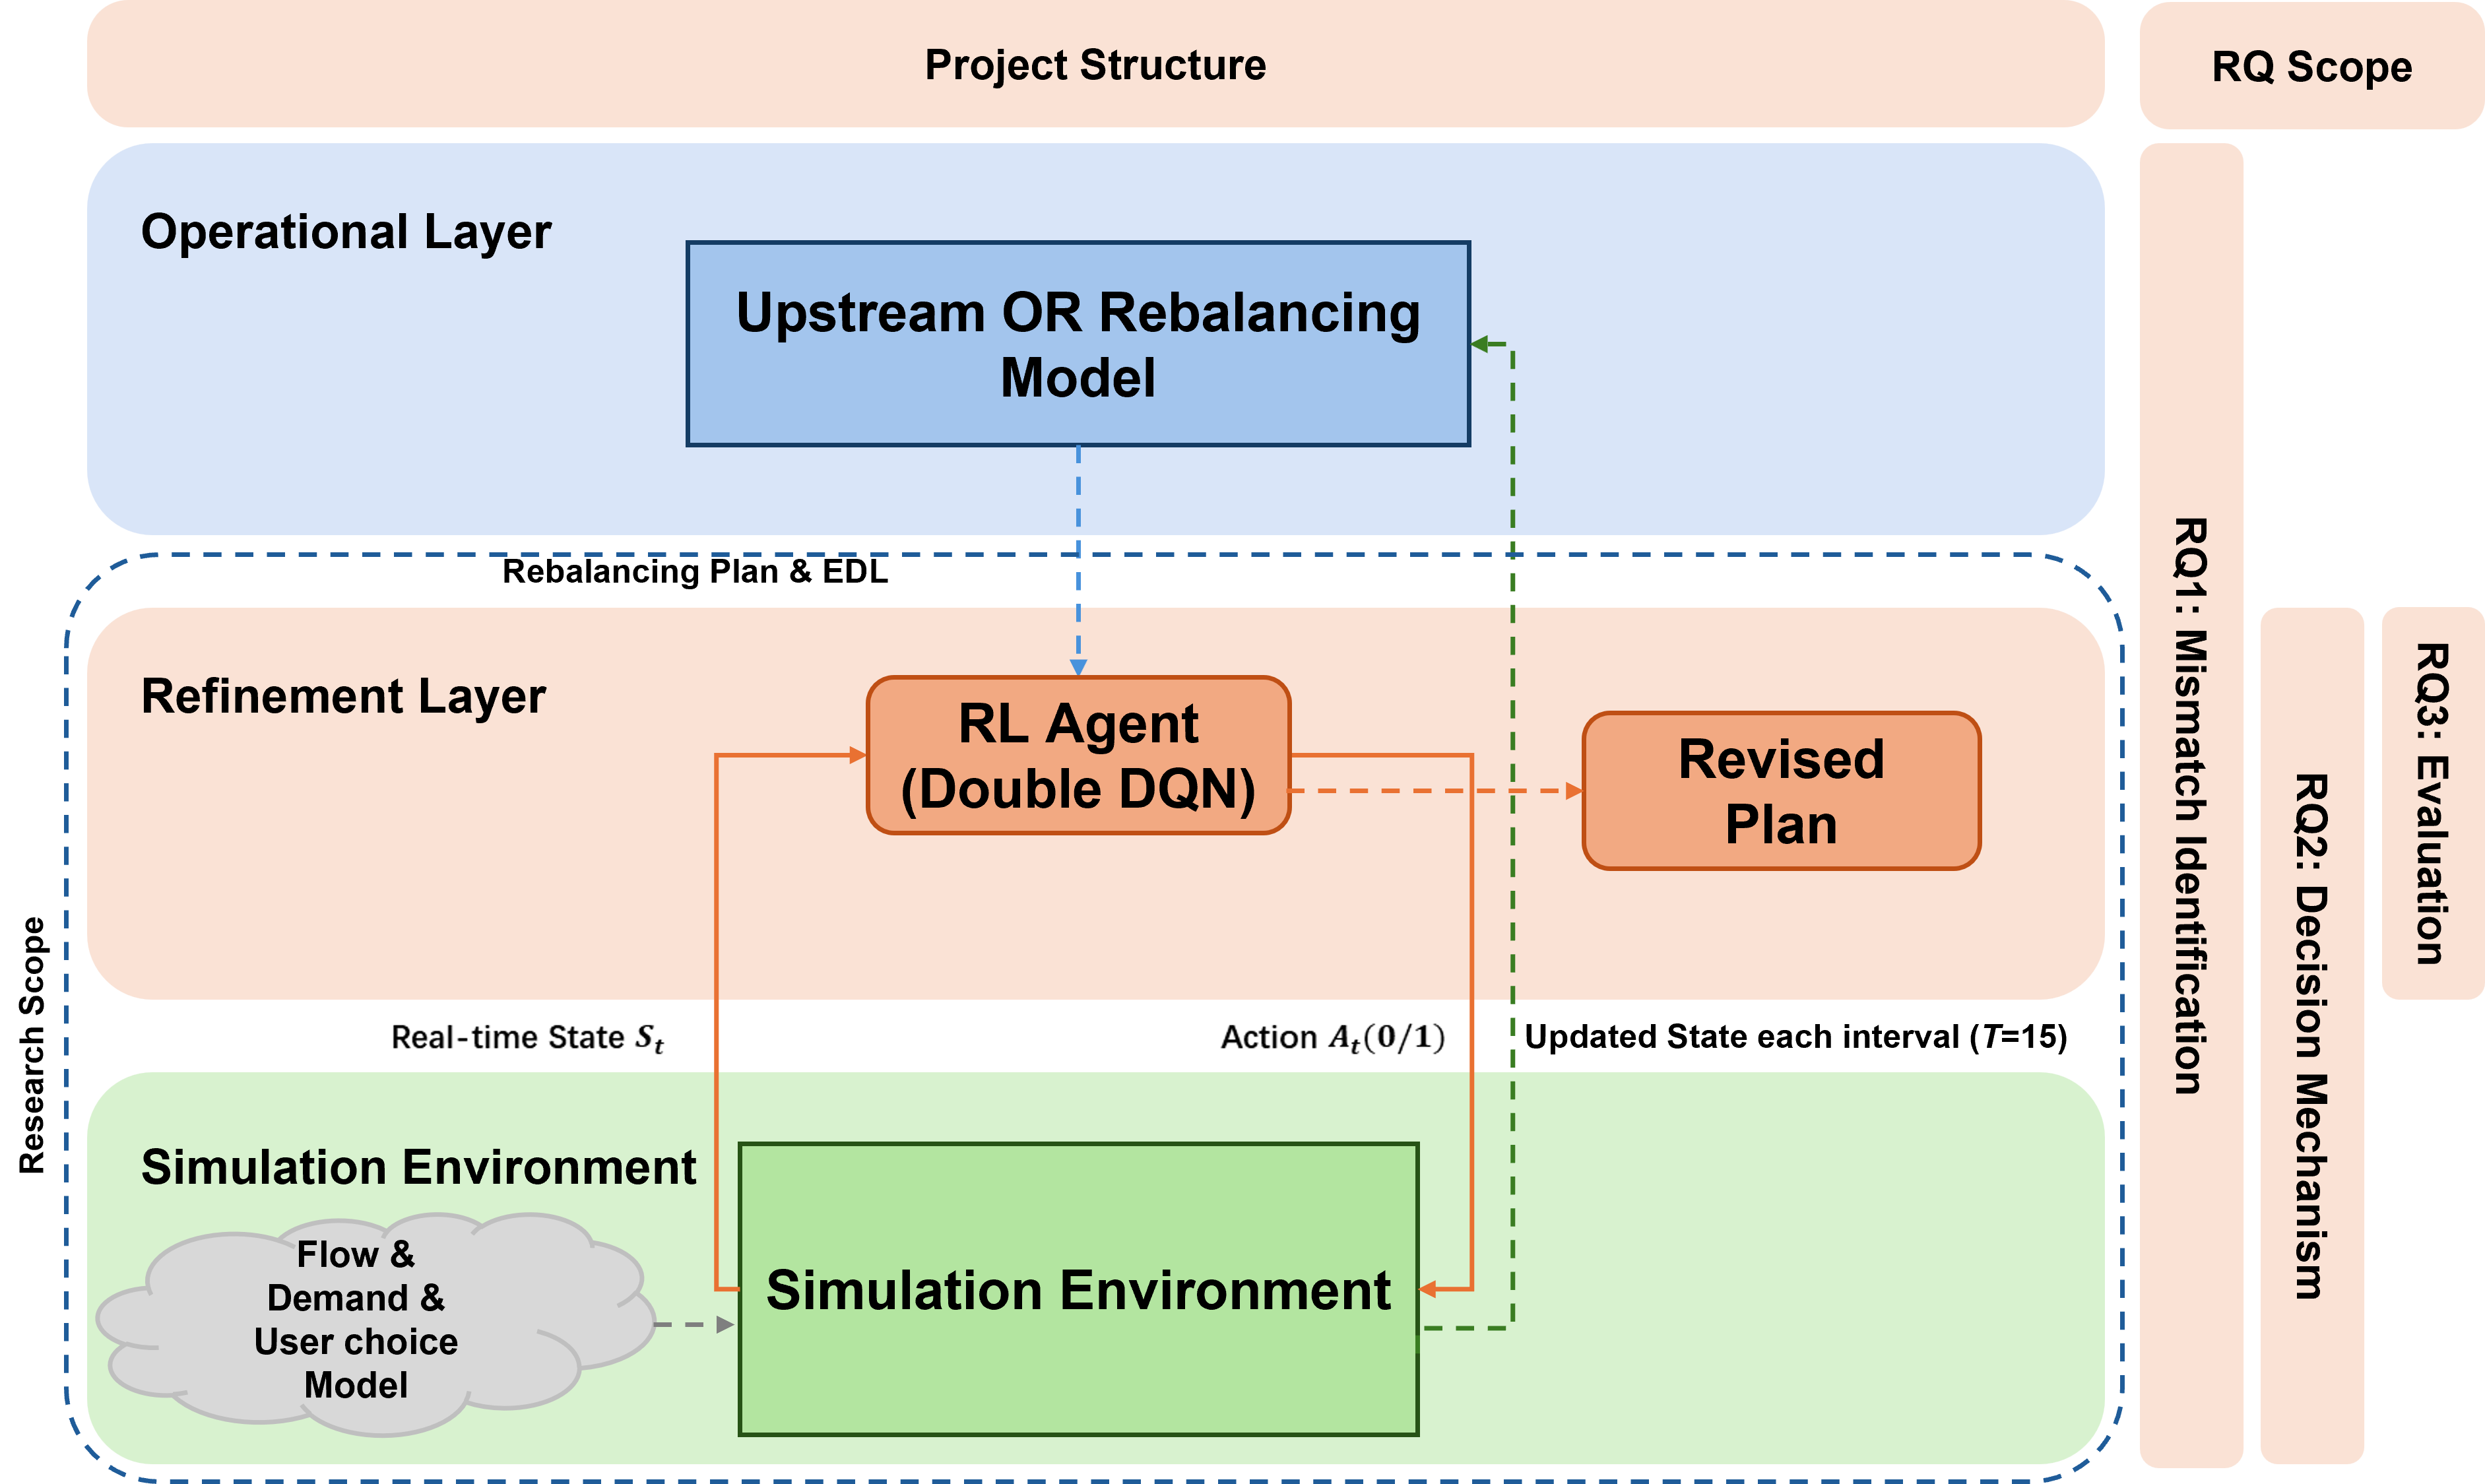
\includegraphics[width=1\textwidth]{figures/figure.png}
    \caption{Layered decision hierarchy and analytical scope of the research questions.}
    \label{fig:decision-hierarchy}
\end{figure}

Figure~\ref{fig:decision-hierarchy} illustrates the layered research structure of the thesis, including the upstream rebalancing model, the trip-level refinement layer, the simulation environment, and the analytical scope of RQ1--RQ3.

The thesis adopts a two-layer decision hierarchy. The upper layer is an interval-based rebalancing model that produces relocation guidance, such as target inventory levels, recommended relocation directions, or candidate relocation trips over a planning horizon. Operating on discretized intervals, this layer provides the global planning logic of the system.

The lower layer is the trip-level execution layer studied in this thesis. Its role is not to recompute the rebalancing plan, but to decide whether guidance from the upper layer should be activated when an eligible trip request arrives. This decision is based on the observed real-time system state and the local execution context. In this way, the upper layer defines relocation intent, while the lower layer determines whether that intent should be implemented for a specific trip.

This separation is central to the scope of the thesis. It keeps the analysis focused on the planning--execution interface rather than expanding into a full redesign of the control architecture. It also makes the research question operationally meaningful: even with a fixed upstream rebalancing model, substantial performance gains may still be achieved through better trip-level execution.

\section{Formal Problem Definition}

The execution problem studied in this thesis is defined at the level of individual eligible trip requests. At each decision epoch, a request arrives in continuous time. For that request, the system observes the current network state, checks whether relocation guidance exists for the request context, and determines whether an incentive should be issued.

The decision input consists of four main elements. First, the observed system state describes zone-level inventory conditions, battery composition, and other operational signals relevant to near-term service performance. Second, the trip request itself provides origin, intended destination, and request timing information. Third, the upstream OR model or rebalancing model may provide a suggested relocation target or indicate that the request belongs to the eligible execution scope. Fourth, uncertainty remains in the form of user acceptance, future realized demand, and evolving resource availability.

Under this setting, the action space is binary: offer or do not offer. If no incentive is offered, the trip proceeds according to its original execution path. If an incentive is offered, the user may either accept the relocation or reject it, and the realized outcome influences the subsequent system state. The objective is to improve service-related outcomes and incentive efficiency by making better execution decisions at the moment of request arrival.

This problem formulation makes the refinement layer event-driven, state-dependent, and stochastic. Decisions are triggered by trip arrivals, their desirability depends on the local system state, and both demand realization and user response remain uncertain even after a decision has been made.

\section{Scope and Delimitations}

The scope of the thesis is intentionally narrow. The study focuses on trip-level selective execution of relocation guidance in a shared e-scooter setting. The upstream OR model or rebalancing model is treated as an external planning input rather than as an object of redesign. Likewise, the incentive mechanism is studied in a simplified binary form, where the operational question is whether to trigger an offer rather than how to optimize a continuous price signal.

Several elements are therefore outside the scope of this thesis. The study does not redesign the upstream OR model, examine continuous incentive pricing, or formulate a full joint optimization of planning and execution. It also does not attempt to solve a wider operational fleet-management problem involving all relocation levers simultaneously, such as truck routing, battery swapping logistics, and joint multi-operator dispatching. The goal is narrower and more precise: to isolate the value of a trip-level execution layer under uncertainty.

This restricted scope keeps the action space interpretable, allows the planning--execution interface to be studied directly, and makes the resulting framework easier to evaluate in simulation. It also aligns with the broader logic of the thesis: the contribution lies in refining execution, not in replacing the entire system architecture.

\section{Mapping of Research Questions to Analysis}

The three research questions introduced in Chapter~\ref{chapter:introduction} map directly onto the analytical structure of the thesis. RQ1 addresses execution mismatch identification by examining how interval-based relocation guidance can diverge from realized trip-level system conditions once stochastic demand, battery-state changes, and local capacity constraints begin to unfold within a planning interval.

RQ2 addresses decision-mechanism design by specifying how the trip-level execution problem should be represented in terms of state, action, uncertainty, and operational objective. This question motivates the formal design of the refinement layer developed in the later methodological chapters.

RQ3 addresses comparative performance evaluation by defining how the proposed execution mechanism will be compared against baseline policies and how resulting changes in service-related outcomes and incentive efficiency will be measured. This evaluation logic supports the empirical chapters that follow.

By structuring the research questions in this way, the thesis maintains a clear progression: identify the operational mismatch, define the trip-level decision problem, and then evaluate whether the proposed mechanism improves execution outcomes.

\section{Chapter Summary}

This chapter has defined the research setting of the thesis in formal terms. It has clarified that the study concerns a free-floating e-scooter system with stochastic demand, battery-dependent vehicle availability, and externally provided relocation guidance. It has also distinguished the upstream OR model or rebalancing model from the downstream trip-level execution layer and specified the scope of the thesis as one of selective execution rather than full planning redesign. With this problem definition in place, the next chapter introduces the methodological framework used to study the proposed execution mechanism.

\chapter{Methodology}
\label{chapter:methodology-overview}

This chapter presents the methodological framework of the thesis. Building on the problem definition in Chapter~\ref{chapter:objectives-problem}, it describes the event-driven simulation environment, the way relocation guidance from the upstream OR model enters the execution layer, and the formulation of the trip-level refinement problem for reinforcement-learning-based evaluation. The emphasis is on the operational logic of the framework rather than on the internal formulation of the upstream rebalancing model.

\section{Methodological Overview}

% \subsection{Layered Framework}

% The methodology follows a layered structure. The upstream layer is an OR model or rebalancing model that produces interval-based relocation guidance. In this thesis, these outputs are treated as external inputs. The downstream layer is a trip-level refinement mechanism that decides whether a relocation suggestion should actually be activated when an eligible trip request is realized. The simulation environment connects these two layers by providing the evolving state of the e-scooter system, the realized demand stream, the user-response model, and the resulting inventory and battery-state transitions.

% This separation is central to the thesis. The refinement layer does not replace the upstream planning layer, does not recompute the OR solution, and does not generate new relocation targets independently. Its role is narrower: given an existing relocation opportunity, it determines whether issuing the incentive is operationally worthwhile under the current realized state. This makes the methodology suitable for studying the planning--execution interface without expanding the thesis into a full redesign of the rebalancing architecture.

Figure~\ref{fig:methodology-workflow} presents the event-driven execution workflow of the framework. It shows how the upstream OR input, the trip-level refinement layer, and the simulation environment interact within a planning interval.

\begin{figure}[H]
    \centering
    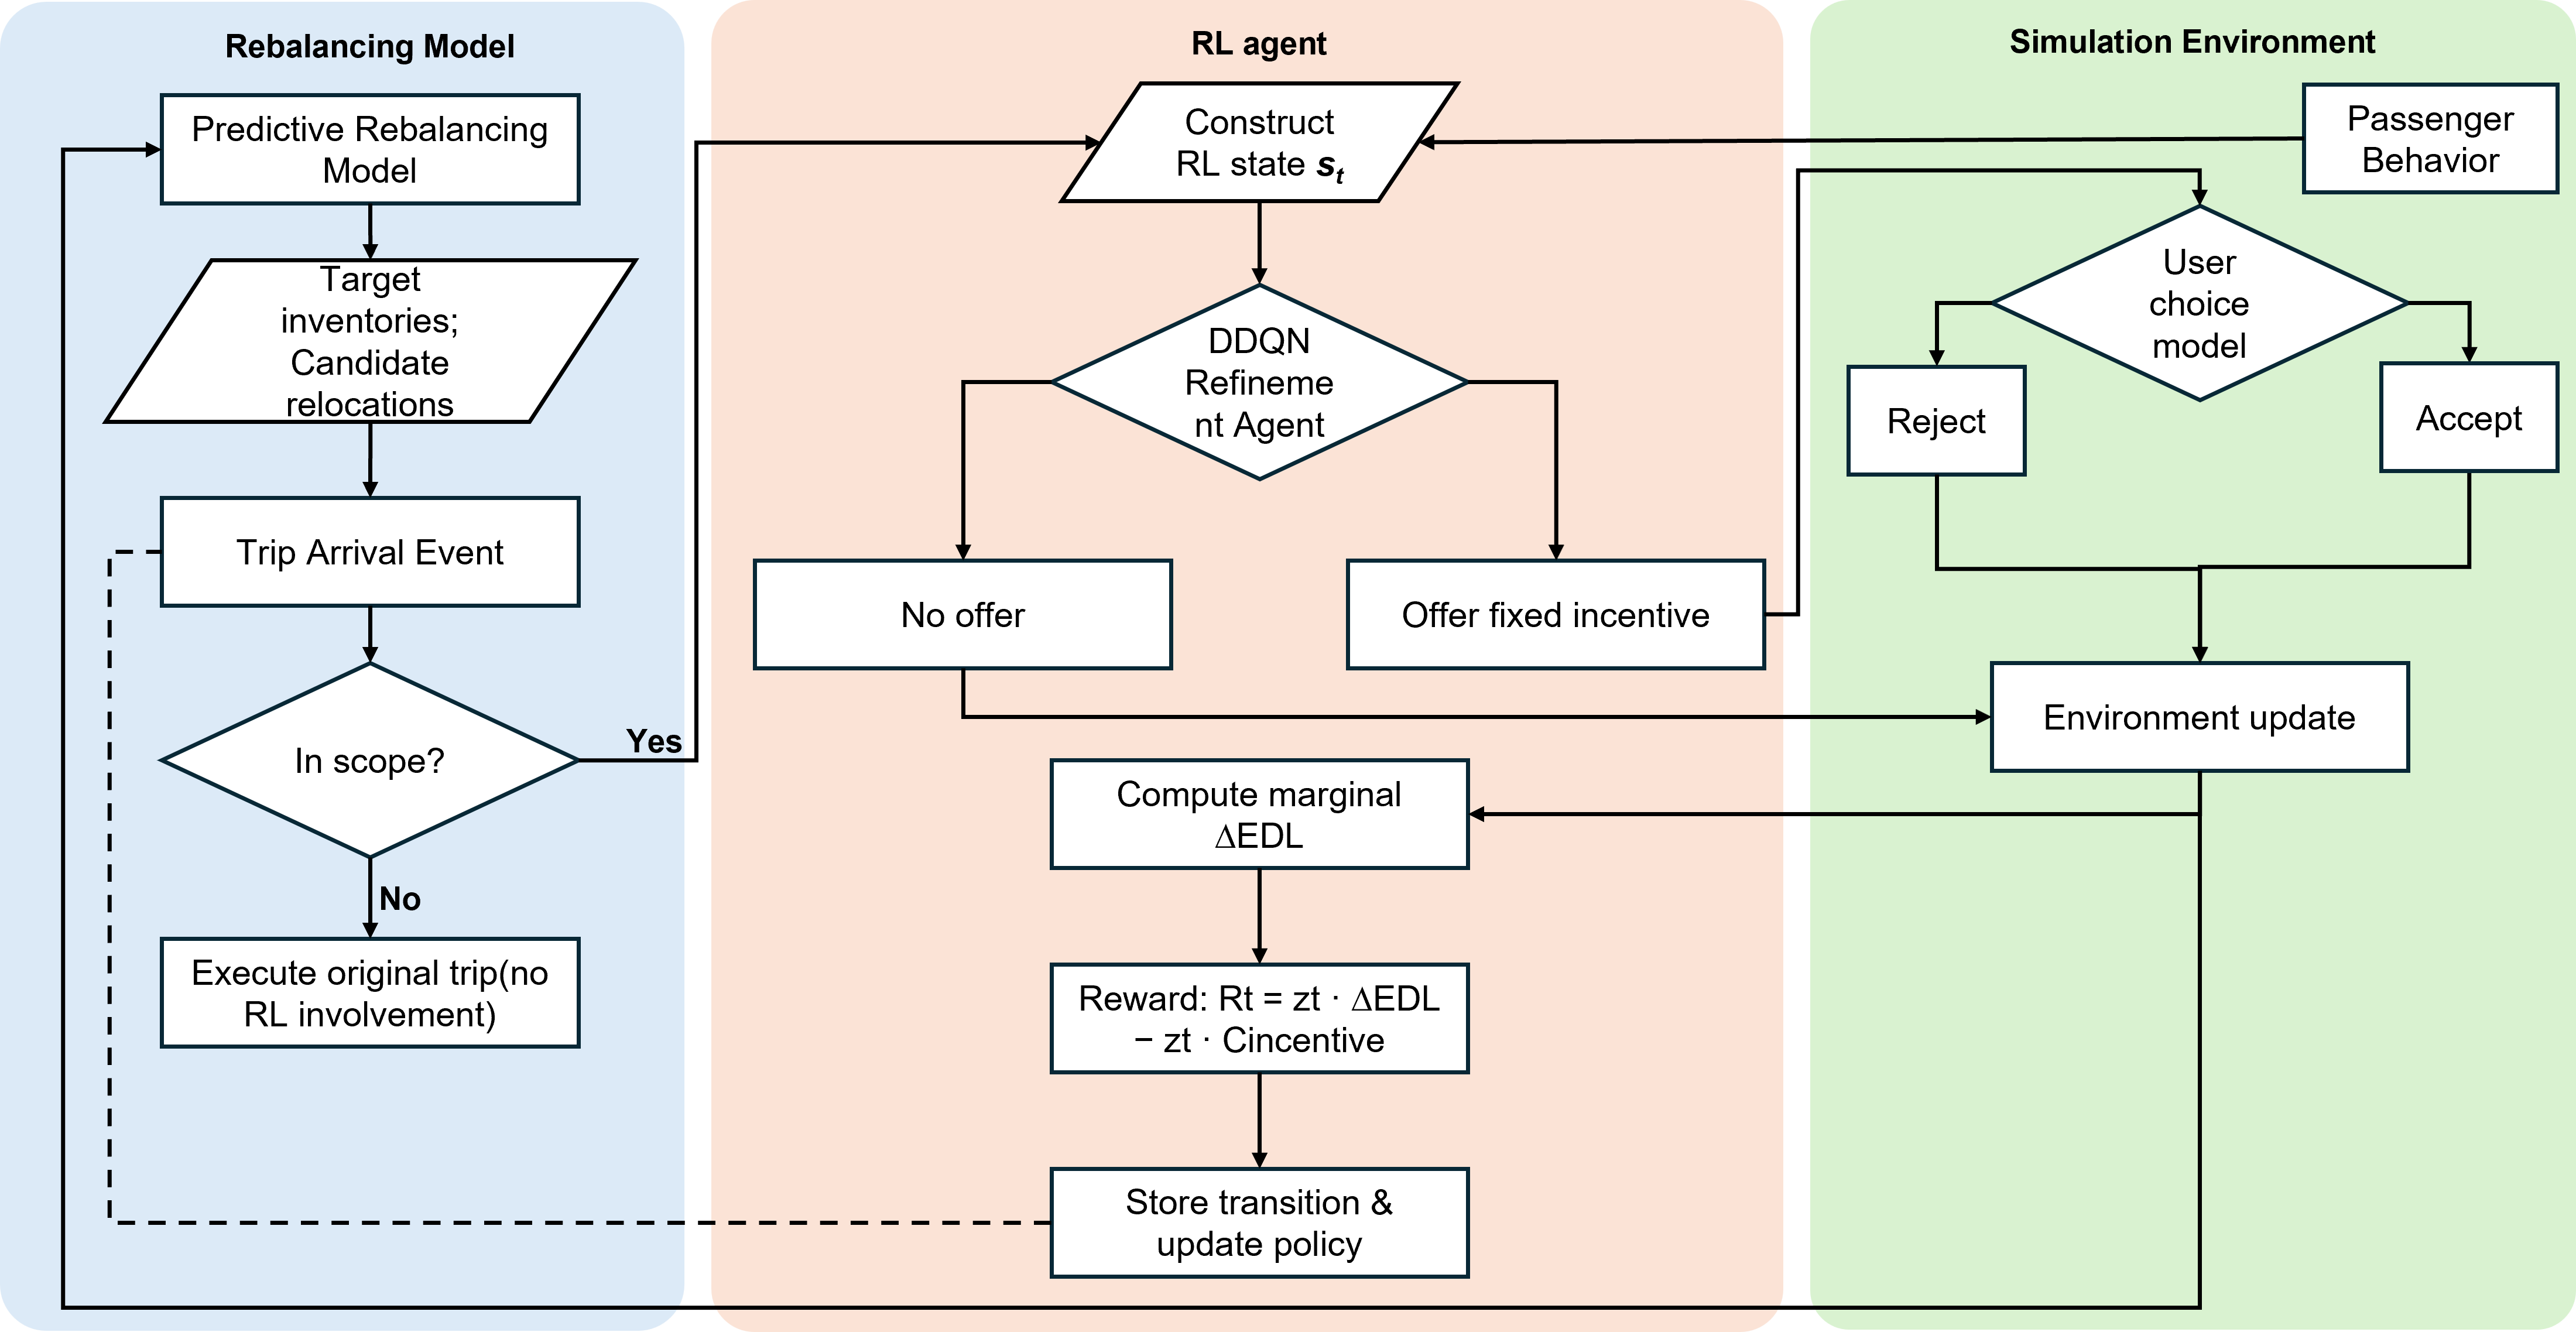
\includegraphics[width=1\textwidth]{figures/agent_structure.png}
    \caption{Event-driven execution workflow linking the upstream rebalancing model, the RL-based refinement agent, and the simulation environment.}
    \label{fig:methodology-workflow}
\end{figure}

The workflow is organized around trip events. A simulation episode begins with a pre-generated stream of trip requests, which are then processed in order of request time. For each arrival, the simulator first queries the external OR interface using the request origin, intended destination, and planning time slot. This determines whether the trip is associated with an eligible relocation opportunity from the upstream rebalancing model.

If no matching relocation opportunity exists, the request proceeds without RL involvement. If a match exists, the simulator does not immediately call the refinement layer. It first checks whether a rentable scooter is available at the origin zone. Requests for which no scooter is available are recorded as supply-related service loss and leave the decision process at that point.

Only requests that satisfy both conditions, namely OR matching and scooter availability, enter the refinement layer. The system state is then assembled from the observed operational context, including temporal, spatial, inventory, and offer-related information. The refinement policy chooses between two actions: do not activate the relocation offer, or activate the fixed incentive associated with the OR recommendation.

After the RL action is determined, the simulator evaluates a single-layer user choice. When no relocation offer is activated, the feasible user actions are to proceed with the original trip or to opt out. When the relocation offer is activated, the feasible user actions are to accept the offered relocation, keep the original destination, or opt out. The final behavioral outcome is thus one of three realized actions: offer, base, or opt\_out.

If the realized choice is offer, the effective destination becomes the recommended destination from the OR input. If the realized choice is base, the trip keeps its original destination. If the realized choice is opt\_out, the request leaves the execution process without being served. Otherwise, the trip is completed through scooter assignment, trip execution, battery-state transition, and an inventory update at the realized destination.


After the trip outcome is known, the simulator records the operational consequences of the decision. These include whether the trip was served, whether a relocation was accepted, and how the local state changed after execution. For RL-enabled runs, the simulator also stores the decision as a temporary transition and completes the reward calculation when the next relevant decision state is observed, or at the end of the episode. This delayed-reward design allows the framework to capture not only the immediate trip outcome, but also realized loss and downstream EDL-related effects that appear between consecutive decision points.

This workflow clarifies the methodological role of the refinement layer. The RL agent does not manage all trips, assign scooters, or generate new relocation targets. Its role is narrower: it decides whether an already available relocation opportunity from the upstream OR model should be implemented for an eligible trip request under the current system state.


\section{Simulation Environment}

The experimental setting is an event-driven simulator for a free-floating shared e-scooter system. The simulator represents the service area as a finite set of geo-fenced zones, tracks zone-level inventory by battery category, processes trip requests in event time, and updates the system state after each served trip. This environment provides the controlled setting in which OR-only execution and OR-plus-RL refinement can be compared.

\subsection{Spatial Representation and Capacity}

The service area is represented as a set of discretized service zones \parencite{momen2025}. Each zone can act as an origin or destination of a trip and is associated with a finite capacity. The primary spatial setup is built from a station-map representation, where zone identifiers are mapped to coordinates and adjacency is derived from walking-distance thresholds. A synthetic grid constructor remains available as a fallback or prototype mode, but it is not the main description of the thesis environment.

At the state level, each zone is represented by a compact inventory tuple: inactive scooters, low-battery scooters, and high-battery scooters. Low- and high-battery scooters are treated as rentable, while inactive scooters are physically present but not serviceable. This distinction is necessary because service availability depends on battery-aware inventory rather than on total fleet count alone. Capacity is also used in the EDL-related state and reward logic, where full and empty states affect expected future service loss.

% \subsection{Demand and Trip Generation}

% Demand enters the simulator through trip requests. Each request contains an origin zone, an intended destination zone, a request time, a trip duration, a trip distance, and a user type. The simulation engine generates requests for an episode in advance and then processes them in time order, preserving event-time dynamics within each planning interval.

% The default demand source for OR/RL experiments is OD-slot sampling based on expected flows. In this mode, expected demand is specified for origin-destination-time combinations and then sampled stochastically during the simulation. Alternative demand sources, including simpler Poisson generation, also remain available. For the RL workflow studied here, OD-slot sampling is especially useful because it allows demand density to be shaped around OR-matched opportunities while keeping the evaluation profile fixed.

\subsection{Trip Generation under Demand Uncertainty}

To simulate passenger arrivals at trip level while preserving consistency with the upstream OR layer, we generate requests from the aggregated OD expectation table and inject stochasticity only in the simulator.  
The OR model itself remains unchanged and still optimizes on aggregated demand inputs.

\paragraph{Mean demand construction.}
Let $\omega_{odt}$ denote the expected number of trips from origin zone $o$ to destination zone $d$ in time slot $t$, derived from the aggregated demand table (\texttt{omega\_h}).  
In the simulator, the slot-level mean is
\begin{equation}
\mu_{odt} = \omega_{odt} \cdot s_g \cdot s_w(t) \cdot s_{od}(o,d,t),
\end{equation}
where $s_g$ is a global scaling factor, $s_w(t)$ is an optional window-specific factor, and $s_{od}(o,d,t)$ is an optional OD-target factor (used for controlled stress/signal settings).

\paragraph{Arrival count distribution.}
A pure Poisson assumption is used as baseline, but the final setting adopts a Negative Binomial (NB2) arrival model to capture over-dispersion observed across days and time periods:
\begin{equation}
N_{odt} \sim \mathrm{NB2}(\mu_{odt}, \phi_t),
\end{equation}
with
\begin{equation}
\mathbb{E}[N_{odt}] = \mu_{odt}, \qquad
\mathrm{Var}(N_{odt}) = \mu_{odt} + \phi_t \mu_{odt}^2.
\end{equation}
Thus, $\phi_t=0$ reduces to the Poisson case, while $\phi_t>0$ increases variance without changing the mean.

\paragraph{Sampling implementation.}
NB2 is implemented via a Gamma--Poisson mixture:
\begin{equation}
\tilde{\lambda}_{odt} \sim \Gamma(k_t,\theta_{odt}), \quad
N_{odt} \sim \mathrm{Poisson}(\tilde{\lambda}_{odt}),
\end{equation}
with
\begin{equation}
k_t=\frac{1}{\phi_t}, \qquad \theta_{odt}=\frac{\mu_{odt}}{k_t},
\end{equation}
which guarantees the NB2 mean--variance structure above.

\paragraph{Dispersion profile calibration.}
Because only aggregated OD averages are available (instead of full day-level OD count sequences), we use a robust proxy calibration for $\phi_t$ by hour:
\begin{enumerate}
\item Compute network-level hourly totals $T(d,h)$ across day-of-week $d$.
\item For each hour $h$, compute coefficient of variation $\mathrm{CV}_h$ over $d$.
\item Map to dispersion using
\begin{equation}
\phi_h = \mathrm{clip}(a\cdot \mathrm{CV}_h + b,\ \phi_{\min},\ \phi_{\max}),
\end{equation}
with default $a=2.0$, $b=0.1$, $\phi_{\min}=0.05$, $\phi_{\max}=5.0$.
\end{enumerate}
The resulting profile is stored as \texttt{nb\_phi\_profile.csv} and loaded at runtime (\texttt{by\_hour} mode).  
This design is configurable and can be replaced by MLE-based estimation once day-level OD counts become available.

\paragraph{Trip-level event generation.}
For each sampled count $N_{odt}$, the simulator creates $N_{odt}$ trip requests by uniformly sampling a request time within slot $t$, fixing the origin and destination to $(o,d)$, drawing trip duration and distance from the existing simulator distributions, and sampling user type from the configured user-type prior.

\paragraph{Rationale.}
This design preserves OR--simulation consistency at the mean level (same aggregated demand source) while providing realistic stochastic variability for RL training and evaluation.  
In summary, OR remains an expectation-level optimizer, and the simulator emulates realized trip uncertainty around that expectation.


\subsection{Fleet and Battery-State Dynamics}

Fleet dynamics are tracked at the scooter level and aggregated to zone-level state variables. When a trip is served, the simulator selects an available scooter from the origin zone, removes it from the origin inventory, applies a trip completion event, updates its battery category, and adds it to the realized destination inventory. Scooter assignment follows scenario-specific rules that are discussed later in the thesis.

Battery evolution is modeled through a Markov transition mechanism over the inactive, low, and high categories \parencite{momen2025}. This allows the simulator to capture the operational fact that a scooter can remain physically present while becoming unavailable for future users. The resulting state transition is therefore not only spatial but also energy-dependent.

\subsection{User Response Modeling}

User behavior is part of the simulation environment rather than part of the RL policy. It is modeled as a single-layer discrete choice process aligned with the choice-model formulation used in the referenced e-scooter studies \parencite{burghardt2025behavioral,momen2025}. When no relocation offer is activated, the user chooses between proceeding with the original trip and opting out. When a relocation offer is activated, the user chooses among accepting the offered relocation, keeping the original destination, and opting out.

For an eligible decision event \(i\), define common user/context attributes
\[
\mathbf{z}_i=
\left[
\text{type}_{25},
\text{prev\_use},
\text{bike},
\text{income\_low},
\text{living\_alone},
\text{living\_shared},
\text{attitude},
\text{range\_anxiety}
\right]_i .
\]
The base and offer utilities are written as
\begin{equation}
\begin{aligned}
V_i^{(\textit{base})}
=\;&
\frac{1}{2}\beta_{ES}
+\beta_{walk}\,walk_i^{base}
+\beta_{unlock}\cdot 1
+\beta_{ride}\,c_i^{base}
+\beta_{batt}\,r_i^{base}
\\
&+
\beta_{type}\,\text{type}_{25,i}
+\beta_{prev}\,\text{prev\_use}_i
+\beta_{bike}\,\text{bike}_i
+\beta_{inc}\,\text{income\_low}_i
\\
&+
\beta_{alone}\,\text{living\_alone}_i
+\beta_{shared}\,\text{living\_shared}_i
+\eta_{att}\,\text{attitude}_i
+\eta_{range}\,\text{range\_anxiety}_i,
\end{aligned}
\end{equation}
\begin{equation}
\begin{aligned}
V_i^{(\textit{offer})}
=\;&
\frac{1}{2}\beta_{ES}
+\beta_{walk}\,walk_i^{offer}
+\beta_{unlock}\cdot 1
+\beta_{ride}\,c_i^{offer}
+\beta_{batt}\,r_i^{offer}
\\
&+
\beta_{type}\,\text{type}_{25,i}
+\beta_{prev}\,\text{prev\_use}_i
+\beta_{bike}\,\text{bike}_i
+\beta_{inc}\,\text{income\_low}_i
\\
&+
\beta_{alone}\,\text{living\_alone}_i
+\beta_{shared}\,\text{living\_shared}_i
+\eta_{att}\,\text{attitude}_i
+\eta_{range}\,\text{range\_anxiety}_i.
\end{aligned}
\end{equation}
The opt-out alternative is the reference utility:
\[
V_i^{(\textit{opt-out})}=0.
\]
The monetary/range sub-terms are
\[
c_i^{base}=p_{ride}\cdot rt_i^{base},
\qquad
c_i^{offer}=p_{ride}\cdot rt_i^{offer}-inc_i,
\]
\[
r_i^{base}=k_{range}\cdot batt_i^{base},
\qquad
r_i^{offer}=k_{range}\cdot batt_i^{offer}.
\]
When no offer is activated, the feasible set is \(\mathcal{A}_i=\{\textit{base},\textit{opt-out}\}\); when an offer is activated, \(\mathcal{A}_i=\{\textit{offer},\textit{base},\textit{opt-out}\}\).

Choice probabilities are computed with a softmax form over the feasible set \(\mathcal{A}_i\):
\[
P_i(a)=\frac{\exp\!\left(V_i^{(a)}\right)}{\sum_{b\in \mathcal{A}_i}\exp\!\left(V_i^{(b)}\right)}, \quad a\in\mathcal{A}_i.
\]
Accordingly, \(\mathcal{A}_i=\{\textit{base},\textit{opt-out}\}\) when no offer is activated, and \(\mathcal{A}_i=\{\textit{offer},\textit{base},\textit{opt-out}\}\) when an offer is activated. The realized user action is then sampled from \(P_i(\cdot)\).

\paragraph{Parameter interpretation.}
The utility parameters are grouped by behavioral meaning.  
\(\beta_{walk}\), \(\beta_{ride}\), and \(\beta_{unlock}\) capture sensitivity to access time and monetary trip cost components; \(\beta_{batt}\) captures the effect of battery-related range utility.  
\(\beta_{type}\), \(\beta_{prev}\), \(\beta_{bike}\), \(\beta_{inc}\), \(\beta_{alone}\), and \(\beta_{shared}\) represent user-attribute and context effects, while \(\eta_{att}\) and \(\eta_{range}\) capture latent attitude and range-anxiety effects.  
The constants \(p_{ride}\) and \(k_{range}\) define the price and range conversion terms used to map trip and battery attributes into utility inputs.  
In this chapter, these terms are defined at model level; the concrete coefficient values and default attribute settings used in experiments are reported in Chapter~7 (Table~\ref{tab:user-model-params}).

Accordingly, the RL policy does not determine the final user choice. It decides only whether the relocation offer is activated, after which the realized user action is sampled from the corresponding choice set.

\section{OR Interface and Refinement Boundary}

\subsection{External OR Interface}

The upstream rebalancing model enters the simulator through an external OR interface. As a result, the simulator does not depend on the internal optimization structure of the upstream model. It consumes only execution-relevant outputs that have already been translated into a standardized relocation table, denoted as \texttt{U\_odit}.

Each row of \texttt{U\_odit} defines one candidate relocation opportunity. The table specifies the origin zone, the original destination zone, the recommended destination zone, the planning time slot, the incentive amount, and the associated relocation quota. At runtime, the simulator queries this table using the realized request origin, intended destination, and request-time slot. If a matching opportunity with remaining quota exists, the request is treated as eligible for refinement-layer intervention. Otherwise, it proceeds outside the OR-guided relocation context.

This interface makes the refinement problem modular. The simulator can evaluate trip-level execution decisions without depending on how the upstream OR model was formulated, calibrated, or solved. The thesis therefore studies the execution consequences of OR-generated guidance rather than the internal mechanics of OR plan generation.

\subsection{Refinement Boundary}

The role of the refinement layer is deliberately narrow. It does not generate relocation intent independently, does not compute new target inventories, and does not re-optimize the upstream plan. Instead, it operates only on relocation opportunities that already exist in the OR input and decides whether a matched opportunity should be activated for a realized trip request.

This boundary is important for the thesis contribution. The proposed policy is not a full rebalancing controller. It does not choose among arbitrary destinations or redesign the global allocation of vehicles across the network. The recommended destination is already fixed by the OR input when the refinement decision is made. The RL policy therefore acts on only one operational degree of freedom: whether to activate or suppress an already available relocation offer.

The same logic applies to quota handling. Quota is defined by the OR input and managed by the OR interface according to the selected quota-consumption rule. The refinement layer does not modify quota values or create additional relocation opportunities. It only interacts with the currently available opportunity and its remaining execution feasibility.

Defining the refinement boundary in this way keeps the research problem well posed. It ensures that the thesis remains focused on selective execution of interval-based relocation guidance rather than drifting into joint planning-and-control optimization. It also makes the later evaluation easier to interpret: any observed difference between OR-only execution and OR-plus-RL execution can be attributed to trip-level activation decisions rather than to changes in the upstream relocation plan itself.


\section{Trip-Level Refinement Problem}

\subsection{Decision Epoch}

The refinement layer faces a binary decision at eligible OR-matched trip events. A decision epoch occurs only when the simulator has identified a relocation opportunity for the arriving request and a rentable scooter is available at the origin zone. This definition is narrower than all trip arrivals and reflects the actual operational role of the refinement layer.

At each such decision epoch, the policy receives a state representation constructed from the current system context. The resulting action is then interpreted as an execution decision: suppress the relocation offer or activate the fixed incentive offer associated with the OR recommendation.

\subsection{State Representation}

The state representation is designed to capture the local execution context of an OR-matched trip event in a compact but operationally meaningful form. Rather than describing the entire network in full detail, the state focuses on the information that is most directly relevant for deciding whether an available relocation opportunity should be activated under the current system conditions.

The state combines five groups of information. First, it includes a temporal feature that indicates the current position of the request within the episode. Second, it contains spatial identity features for the origin, the original destination, and the recommended destination associated with the matched OR opportunity. Third, it includes battery-aware inventory features for these same three zones. Fourth, it contains EDL-related features that summarize the local expected-loss context at the decision time. Fifth, it includes trip-level and offer-level attributes that characterize the immediate operational trade-off of activating the relocation option.

To avoid notation conflict with decision-step indexing, this thesis uses \(R_i\) for the recommended destination zone associated with decision step \(i\), while \(i\) itself always denotes the decision-step index.

Table~\ref{tab:state-features} summarizes the variables included in the current state vector.

\begin{table}[H]
\centering
\caption{State variables used in the current trip-level refinement policy.}
\label{tab:state-features}
\begin{tabular}{p{3.2cm}p{5.4cm}p{5.2cm}}
\toprule
\textbf{Feature group} & \textbf{Variables} & \textbf{Meaning} \\
\midrule
Temporal context
& \texttt{slot\_norm}
& Normalized position of the current request within the episode, derived from the planning slot. \\

Spatial identity
& \texttt{origin\_id}, \texttt{destination\_id}, \texttt{recommended\_id}
& Normalized identifiers of the origin zone, original destination zone, and recommended destination zone. \\

Origin-zone inventory
& \texttt{o\_n}, \texttt{o\_l}, \texttt{o\_h}
& Normalized inactive, low-battery, and high-battery scooter counts at the origin zone. \\

Original-destination inventory
& \texttt{d\_n}, \texttt{d\_l}, \texttt{d\_h}
& Normalized inactive, low-battery, and high-battery scooter counts at the original destination zone. \\

Recommended-destination inventory
& \texttt{r\_n}, \texttt{r\_l}, \texttt{r\_h}
& Normalized inactive, low-battery, and high-battery scooter counts at the recommended destination zone. \\

EDL context
& \texttt{edl\_o}, \texttt{edl\_d}, \texttt{edl\_r}
& EDL-related features for the origin, original destination, and recommended destination at the decision time. \\

Trip and offer attributes
& \texttt{rt\_base}, \texttt{rt\_offer}, \texttt{walk\_extra}, \texttt{incentive}
& Base ride time, ride time under relocation, additional walking time, and fixed incentive amount. \\

Resource context
& \texttt{quota\_remaining}, \texttt{budget\_remaining}
& Remaining quota of the matched relocation opportunity and remaining budget-related context passed to the decision layer. \\
\bottomrule
\end{tabular}
\end{table}


Taken together, the state representation is intentionally local, structured, and decision-oriented. It combines temporal position, spatial identity, battery-aware local inventory, EDL signals, and offer attributes into a single vector that is informative enough for trip-level selective execution while avoiding the complexity of a full-network end-to-end representation.



\subsection{Action Space}

The action space is binary. Action 0 suppresses the relocation offer, so the user faces the no-offer choice set and may either proceed with the original trip or opt out. Action 1 activates the fixed relocation incentive, so the user faces the offer-enabled choice set and may choose the relocation option, keep the original destination, or opt out.

This restricted action space is intentional. It keeps the refinement mechanism interpretable, avoids turning the thesis into a continuous pricing problem, and aligns the policy with the core operational question: whether an existing relocation suggestion should be activated for a realized trip request.


\subsection{Sources of Uncertainty}

The execution outcome remains uncertain even after the binary action is selected. User response is one source of uncertainty, because the realized behavioral outcome depends on the choice set induced by the RL action and may end in offer, base, or opt\_out. Future trip arrivals are stochastic under the OD-slot demand process. Battery transitions and subsequent inventory evolution also affect future service availability. As a result, the same relocation suggestion may have different operational value depending on the realized state when the trip arrives.

\section{RL Formulation and Policy Logic}

\subsection{Sequential Decision Perspective}

The refinement problem is formulated as a sequential decision problem. Each eligible decision produces a state, an action, a realized outcome, and a transition to a later decision state. This perspective is appropriate because an accepted relocation affects not only the current trip but also future inventory distribution, battery composition, and service availability at later decision times.

The learning setup uses a value-based binary policy. The RL agent is a Double Deep Q-Network (DDQN), which is well suited to the low-dimensional discrete action space and helps reduce the overestimation bias associated with standard DQN. The agent therefore serves as a selective execution policy rather than replacing the upstream OR model.

\subsection{Reward Design}

The reward evaluates trip-level execution decisions in terms of both their immediate operational consequences and their expected downstream effect on system performance. The aim is not to maximize the number of issued offers, but to activate relocation opportunities only when they are likely to improve service-related outcomes while avoiding unnecessary incentive expenditure.

One design choice is to compute reward in delayed form rather than assign it immediately at the moment of action selection. This is necessary because the operational effect of an execution decision is not fully observable at the instant when the offer is activated or suppressed. Some consequences emerge only after the trip outcome is realized and subsequent system evolution reveals whether service loss occurred before the next relevant decision point. The simulator therefore stores each RL decision as a pending transition and finalizes its reward when the next RL decision state becomes available, typically at the next offer opportunity, or at the end of the episode.

The reward combines five components: a realized-loss term, an EDL-improvement term, an acceptance incentive term, a realized-cost term, and a rejection penalty. In compact form, the reward is defined as
\begin{equation}
    r_i
    =
    - w_L \widetilde{L}_i
    +
    w_E \widetilde{\Delta EDL}_i
    +
    \beta_a Acc_i
    -
    \beta_c Cost_i
    -
    \beta_r Rej_i.
\end{equation}

Here, \(L_i\) is the realized no-supply loss over the decision window from decision step \(i\) to the next decision step (or episode end), restricted to the three involved zones \(O_i\), \(D1_i\), and \(R_i\). \(\Delta EDL_i\) is the expected-demand-loss difference induced by the realized action outcome under the fixed OR guidance. \(Acc_i\in\{0,1\}\) indicates whether the relocation option is realized, \(Cost_i\) is realized incentive payout (counted only when relocation is realized), and \(Rej_i\in\{0,1\}\) indicates activated-but-not-accepted outcomes. The coefficients \(w_L,w_E,\beta_a,\beta_c,\beta_r\) control the relative contribution of these components.

To stabilize training signals across episodes, the realized-loss and EDL-improvement components are normalized and clipped as
\begin{equation}
\widetilde{L}_i
=
\mathrm{clip}\!\left(
\frac{L_i}{L_{ref}},\,0,\,1
\right),
\end{equation}
\begin{equation}
\widetilde{\Delta EDL}_i
=
\mathrm{clip}\!\left(
\frac{\Delta EDL_i}{E_{ref}},\,-1,\,1
\right),
\end{equation}
where \(L_{ref}>0\) and \(E_{ref}>0\) are scaling constants, and
\[
\mathrm{clip}(x,a,b)=\min\{\max(x,a),\,b\}.
\]

The first component, \(L_i\), captures realized short-horizon service loss between two consecutive refinement decisions. Let \(\tau_i\) denote the event time of decision step \(i\). Then \(L_i\) is counted over the event window \((\tau_i,\tau_{i+1}]\), or until episode end if no subsequent decision occurs. The counting scope is restricted to the three zones involved in the current decision context: origin \(O_i\), original destination \(D_i\), and recommended destination \(R_i\). This term counts realized no-supply loss events (rather than user opt-out events), and therefore reflects operational deterioration in available service capacity.

The second component, \(\Delta EDL_i\), captures the change in expected demand loss induced by the realized action outcome. This term compares cumulative EDL under a baseline no-relocation counterfactual with cumulative EDL under the realized post-decision state over the fixed look-ahead horizon (2 hours). A positive value indicates that the realized execution outcome is expected to reduce future demand loss relative to not activating relocation.

The normalization anchors \(L_{ref}\) and \(E_{ref}\) are numerical scaling references for comparability and stability, not physical constants. In implementation, both are calibrated from decision-level samples collected across many episodes and seeds using high quantiles (current setup: P95). Specifically, \(L_{ref}\) is estimated from the sample distribution of \(L_i\), and \(E_{ref}\) from \(|\Delta EDL_i|\), with lower-bound guards to avoid degenerate scaling in sparse regimes.

The third component, \(Acc_i\), rewards behaviorally effective activations when the user chooses the offered relocation option (\(Acc_i=1\) if accepted, otherwise \(0\)). The fourth component, \(Cost_i\), represents realized incentive expenditure. Incentive cost is counted only when the relocation option is actually chosen, rather than whenever an offer is only activated. This choice reflects the operational fact that financial payout is incurred only when the user accepts the offered relocation.

The fifth component, \(Rej_i\), penalizes activated offers that do not result in the relocation option being chosen (\(Rej_i=1\) for activated-but-not-accepted offers, otherwise \(0\)). This includes cases where the offer is activated but the realized user choice is not \textit{offer} (i.e., \textit{base} or \textit{opt-out}). This term discourages the policy from activating relocation offers that are unlikely to be behaviorally effective.

Taken together, the reward design reflects the core logic of the refinement layer. The policy should prefer decisions that reduce short-term realized loss, improve future expected demand-loss conditions, activate behaviorally effective offers, avoid unnecessary incentive payout, and refrain from activating offers that are unlikely to be effective. In the current baseline setup, \(w_L=w_E=0.5\), while \(\beta_a\), \(\beta_c\), and \(\beta_r\) are tuned through sensitivity analysis.


\subsection{Training and Evaluation Interface}

The training and evaluation interface assesses the refinement layer as an execution policy operating on top of externally provided rebalancing guidance. In this framework, the upstream OR input remains fixed, while the trip-level policy is trained and evaluated through repeated simulation episodes. This makes it possible to isolate the value of selective execution without conflating it with changes in the planning layer.

From a learning perspective, each episode consists of a sequence of realized trip events processed in event time. Whenever an eligible relocation opportunity arises, the current system state is translated into a policy input, an execution action is selected, and the resulting transition is recorded for learning or evaluation. The simulator thus provides the interaction environment, while the refinement policy is the only component that changes across training and policy-comparison runs.

The training interface is therefore based on repeated environment rollouts under controlled demand and OR-input conditions. During training, the policy explores the action space through stochastic action selection, while observed transitions are stored and used to update the value function. During evaluation, the learned policy is executed without exploratory noise so that its decision behavior can be compared consistently against non-learning baselines. This distinction matters because the objective of the thesis is not only to learn a policy, but also to assess whether the learned execution rule improves operational outcomes relative to simpler alternatives.

Eligible relocation opportunities may be sparse under the target demand distribution. The broader training interface therefore allows different demand-density settings for policy development and final assessment. In particular, a denser demand configuration can be used to expose the policy to more matched relocation opportunities during training, while the final evaluation remains fixed on the target distribution of interest. This does not change the decision problem itself; it addresses the practical issue that sparse decision opportunities can weaken the learning signal if the policy is trained only under the final evaluation distribution.

The evaluation interface compares policies under identical simulation conditions, including the same OR input structure, the same demand-profile specification, and controlled seed schedules. This ensures that differences in observed performance can be attributed to the execution policy rather than to changes in the upstream guidance or the simulation configuration. The main evaluation outputs are therefore interpreted as comparative execution outcomes, not as evidence that the OR plan itself has improved.

Overall, the training and evaluation interface has two purposes: it provides a reproducible procedure for fitting a trip-level execution policy within the proposed framework, and it establishes a fair comparison setting in which OR-only execution and OR-guided refinement policies can be assessed on the same operational basis.


\section{Reproducibility and Configuration Logic}

The methodology is organized in a configurable simulation workspace. Random seeds, planning intervals, episode horizons, OR input paths, demand-source settings, omega sampling profile parameters, reward coefficients, and RL hyperparameters are specified explicitly through configuration files or command-line overrides. This structure allows the same core simulator to be used for OR-only baselines, single-stage RL training, and multi-profile evaluation.

The default OR/RL demand path uses OD-slot expected flows with profile scaling during the simulation. Replay-based demand remains available, but it is not the default for the RL protocol used in this thesis. This distinction is important for reproducibility because the experimental protocol must specify not only the simulator but also the demand distribution under which the policy is trained and evaluated.

The simulator also records transition-level information for RL analysis, including state, action, next state, reward, accepted flag, rejected flag, EDL change, realized loss, and cost term. These logs support later experimental comparison and help diagnose whether the refinement layer is learning from a sufficient number of decision opportunities.

\section{Chapter Summary}

This chapter has presented the methodology as an event-driven execution framework that connects external OR guidance, a battery-aware e-scooter simulation environment, a single-layer user choice model, and a DDQN-based binary refinement policy. The key methodological boundary is that the RL agent does not generate relocation plans or alternative destinations. Instead, it decides only whether an already available OR relocation opportunity should be activated at an eligible trip event.

The chapter also formalized the simulator-side decision logic: only OR-matched requests with available rentable scooters enter the refinement decision point; user behavior is then realized through one-step choice among feasible actions (\textit{offer/base/opt-out}); and system dynamics are updated through trip execution, battery transition, and zone inventory updates.

For learning, the refinement layer is formulated as a sequential decision process with delayed transition finalization and a hybrid reward that combines realized service-loss feedback, EDL-improvement signal, realized incentive cost, and rejection penalty. Together, these design choices provide a reproducible and modular basis for comparing OR-only execution with OR+RL selective execution in the next chapter.

\chapter{Experimental Design}

This chapter defines the experimental protocol used in this thesis. The purpose is to evaluate whether a trip-level refinement layer can improve the execution quality of OR-guided relocation decisions under stochastic demand. To keep the comparison interpretable, the upstream OR plan is fixed and only downstream execution logic is changed.

\paragraph{Placeholder Convention}
Structured placeholders use angle-bracket tokens for later replacement, for example \texttt{\detokenize{<S1\_RL\_SERVICE\_RATE\_MEAN>}} and \texttt{\detokenize{<TAB\_S1\_FINAL>}}.

\section{Evaluation Logic and Policy Comparison}

The evaluation is designed around a layered-control perspective. The OR model provides interval-based relocation opportunities, while the refinement layer decides whether those opportunities should be activated for realized trip events. Under this setup, observed differences can be attributed to execution decisions rather than changes in planning itself.

The policy comparison includes two fixed references and one learned policy in one unified evaluation run: \textit{no-offer}, \textit{always-offer}, and \textit{checkpoint}. Here \textit{checkpoint} denotes the learned RL policy loaded from the selected model checkpoint and executed greedily at evaluation time.
In the current execution interface, \textit{always-offer} is used as the operational counterpart of OR-only execution, because OR suggestions are not suppressed at the trip-execution layer.

\section{Shared Environment and Common Settings}

All policies are evaluated in the same event-driven simulator, with the same OR input table, battery transition model, and user behavior module. A request enters the refinement decision boundary only when it matches a valid OR record and remains operationally feasible in the current state.

The OR interface is represented by a standardized \(U_{odit}\) table, where each record specifies origin, original destination, recommended destination, planning slot, incentive value, and remaining execution quota. The refinement layer does not create new relocation targets and does not redesign OR outputs. It only decides whether a currently available OR recommendation should be activated.

Each episode is defined as a two-hour horizon (\(120\) minutes), and planning slots are aligned to \(15\)-minute intervals for OR matching and EDL timing. Trips are processed in event time inside each episode.

To keep terminology stable across chapters, this thesis uses three evaluation profiles: \textit{main}, \textit{sparse}, and \textit{dense}.  
All three profiles share the same simulator logic, OR input structure, user-choice model, battery-transition model, and policy interface.  
Their only difference is the demand-sampling intensity applied in simulator-side trip realization.

The profile definitions are:
\begin{itemize}
\item \textbf{\textit{main}}: baseline profile used for model training and primary result reporting.
\item \textbf{\textit{sparse}}: lower-demand stress profile used to test policy behavior under fewer matched opportunities.
\item \textbf{\textit{dense}}: higher-demand stress profile used to test policy behavior under heavier event pressure.
\end{itemize}

In implementation, the three profiles are instantiated by different scaling settings on top of the same OD expectation source and NB2 arrival mechanism.  
This means profile changes do not alter upstream OR optimization logic; they only change downstream realized trip exposure in the simulator.


\subsection{Trip-Arrival Uncertainty Setting Used in This Chapter}

Trip-arrival uncertainty follows the methodology introduced in Chapter~4. In this chapter, realized trips are generated from OD-slot expected demand using the NB2 setting (rather than pure Poisson), with hourly dispersion profile loading (\texttt{by\_hour} mode). OR inputs and OR optimization logic remain unchanged.

When sampling-profile scaling is applied, it is used only in the simulator-side trip realization process for training/evaluation exposure control. It does not alter the fixed \(U_{odit}\) plan content. All scaling factors and uncertainty-mode settings are logged per run for reproducibility.
The scaling follows the Chapter~4 formulation:
\[
\mu_{odt}^{(sim)}=\omega_{odt}\cdot s_g \cdot s_w(t)\cdot s_{od}(o,d,t),
\]
where \(s_g\) is the global demand multiplier, \(s_w(t)\) is the window multiplier, and \(s_{od}(o,d,t)\) is the OD-target multiplier.

For this thesis version, profile mappings are fixed as:
\begin{itemize}
\item \textbf{\textit{sparse}}: \texttt{global\_scale=1.0}, \texttt{window\_scale=2.0}, \texttt{od\_target\_scale=5.0}
\item \textbf{\textit{main}}: \texttt{global\_scale=1.5}, \texttt{window\_scale=4.0}, \texttt{od\_target\_scale=8.0}
\item \textbf{\textit{dense}}: \texttt{global\_scale=1.8}, \texttt{window\_scale=5.0}, \texttt{od\_target\_scale=10.0}
\end{itemize}
The active time window is \texttt{slot 0--7}. The OD-target multiplier is applied only to the configured target OD subset. These profile settings change realized trip intensity only; they do not modify OR output, OR interface semantics, or OR planning logic.

\section{Scenario 1: Binary Offer Activation}

\subsection{Decision Scope}

Scenario 1 uses a binary action space:
\[
a_i \in \{0,1\},
\]
where \(a_i=0\) suppresses relocation activation and \(a_i=1\) activates the fixed OR offer at decision step \(i\). The policy is called only at eligible OR-matched events with rentable supply at origin.

In this scenario, scooter assignment remains deterministic (highest-battery-first), so the RL layer controls only activation and not vehicle selection.

\subsection{State Representation}

The Scenario 1 state is a compact execution-context vector defined at each eligible event. It includes: temporal position in the episode, origin/destination/recommended zone identifiers, battery-aware inventory composition at these zones, EDL-related local context, trip-offer attributes (ride-time difference, walking-time difference, incentive amount), and resource context (remaining quota and budget signal).

This representation is intentionally scoped to the refinement boundary. It excludes planning-layer internals to preserve modularity between OR planning and RL execution.

\subsection{User Behavior and Outcome Realization}

User response is modeled as a single-layer discrete choice process. When no offer is activated, the feasible outcomes are \textit{base} or \textit{opt-out}. When an offer is activated, the feasible outcomes are \textit{offer}, \textit{base}, or \textit{opt-out}. The final realized action is sampled from utility-based probabilities.

This design ensures that RL decides activation only, while final behavioral outcome remains stochastic and environment-driven.

\begin{table}[H]
\centering
\caption{User model parameters used in this thesis experiments (Scenario 1).}
\label{tab:user-model-params}
\begin{tabular}{p{4.5cm}p{3.5cm}p{6.0cm}}
\toprule
\textbf{Parameter} & \textbf{Value} & \textbf{Meaning} \\
\midrule
\(\beta_{ES}\) & \(10.514\) & Alternative-specific constant component (shared as \(0.5\beta_{ES}\) in base/offer utility). \\
\(\beta_{walk}\) & \(-0.342\) & Walking-time sensitivity. \\
\(\beta_{unlock}\) & \(-1.419\) & Unlock-fee coefficient. \\
\(\beta_{ride}\) & \(-25.147\) & Ride-cost coefficient. \\
\(\beta_{batt}\) & \(0.27\) & Battery/range utility coefficient. \\
\(\beta_{type}\) & \(-1.02\) & Vehicle-type attribute coefficient. \\
\(\beta_{prev}\) & \(-1.79\) & Previous-use attribute coefficient. \\
\(\beta_{bike}\) & \(-2.21\) & Bike-ownership attribute coefficient. \\
\(\beta_{inc}\) & \(-1.18\) & Low-income attribute coefficient. \\
\(\beta_{alone}\) & \(1.21\) & Living-alone attribute coefficient. \\
\(\beta_{shared}\) & \(-0.86\) & Living-shared attribute coefficient. \\
\(\eta_{att}\) & \(0.82\) & Environmental-attitude latent term coefficient. \\
\(\eta_{range}\) & \(-0.58\) & Range-anxiety latent term coefficient. \\
\midrule
\(p_{ride}\) & \(0.30\) EUR/min & Ride-price constant in cost term \(c^{base},c^{offer}\). \\
\(k_{range}\) & \(0.6\) km/\% & Battery-to-range conversion in \(r^{base},r^{offer}\). \\
\(inc_i\) (fixed offer) & \(1.0\) EUR & Incentive amount used in offer alternative. \\
\midrule
\(\text{type}_{25}\) & \(1\) & Default user attribute in simulation. \\
\(\text{prev\_use}\) & \(1\) & Default user attribute in simulation. \\
\(\text{bike}\) & \(0\) & Default user attribute in simulation. \\
\(\text{income\_low}\) & \(0\) & Default user attribute in simulation. \\
\(\text{living\_alone}\) & \(0\) & Default user attribute in simulation. \\
\(\text{living\_shared}\) & \(0\) & Default user attribute in simulation. \\
\(\text{attitude}\) & \(0.0\) & Default user latent attribute in simulation. \\
\(\text{range\_anxiety}\) & \(0.0\) & Default user latent attribute in simulation. \\
\bottomrule
\end{tabular}
\end{table}
The coefficient set follows the referenced behavioral-model literature \parencite{burghardt2025behavioral,momen2025}, while the experiment-specific constants/defaults are fixed to the current simulator configuration for reproducibility.

\subsection{Reward Design}

Scenario 1 uses a delayed hybrid reward:
\[
r_i
=
w_E\widetilde{\Delta EDL}_i
-
w_L\widetilde{L}_i
+
\beta_a Acc_i
-
\beta_c Cost_i
-
\beta_r Rej_i.
\]

The normalized terms are:
\[
\widetilde{L}_i
=
\mathrm{clip}\!\left(\frac{L_i}{L_{ref}},0,1\right),\qquad
\widetilde{\Delta EDL}_i
=
\mathrm{clip}\!\left(\frac{\Delta EDL_i}{E_{ref}},-1,1\right).
\]

Reward is finalized when the next relevant decision state is observed (or at episode end), so that both immediate and short-horizon downstream effects are reflected in the transition target. For \(L_i\), the realized-loss window is event-based: from decision step \(i\) to the next decision step (or episode end), and only no-supply losses in \(O_i\), \(D1_i\), and \(R_i\) are counted. In this setup, \(Acc_i\) and \(Rej_i\) are binary outcome variables for acceptance and activated-but-not-accepted cases, respectively, while incentive cost is accounted for realized acceptance events.

The normalization anchors \(L_{ref}\) and \(E_{ref}\) are calibrated from decision-level samples across episodes (current setup: P95 with lower-bound guards). \(L_{ref}\) is estimated from the empirical distribution of \(L_i\), and \(E_{ref}\) from \(|\Delta EDL_i|\). They are numerical anchors for scale comparability and stability, not physical constants.

\subsection{Final Training and Evaluation Protocol}

This subsection defines the final protocol used to train and evaluate the Scenario~1 refinement policy.  
The protocol is designed to keep policy comparison fair, preserve reproducibility, and clearly separate primary performance reporting from robustness testing.

\paragraph{Step 1: Training profile and learning setup.}
The RL policy is trained under the \textit{main} demand profile only.  
Scenario~1 uses a binary action space, where the policy decides whether to activate or suppress an OR-matched offer at each eligible decision event.  
Eligibility requires (i) a valid OR match in the current slot and (ii) rentable scooter availability at the origin zone.


\paragraph{Step 2: Checkpoint selection.}
During training, checkpoints are saved at fixed intervals and at the end of training.  
The final model used for policy comparison is selected from this checkpoint sequence according to the predefined run protocol (same seed range and profile assumptions).  
After selection, the checkpoint is frozen and reused across all evaluation profiles to avoid checkpoint-specific bias.

\paragraph{Step 3: Three-profile evaluation.}
The selected checkpoint is evaluated under three profiles:
\begin{itemize}
\item \textit{main}: primary reporting profile;
\item \textit{sparse}: low-demand stress profile;
\item \textit{dense}: high-demand stress profile.
\end{itemize}

All profile changes are applied only to simulator-side trip realization intensity.  
The OR output structure and OR interface remain fixed across profiles.  
Therefore, profile variation tests execution robustness under demand-shift conditions, not changes in planning logic.

\paragraph{Step 4: Three-policy comparison in each profile.}
Within each profile, three policies are evaluated side-by-side:
\begin{itemize}
\item \textit{no-offer}: always suppress activation at decision points;
\item \textit{always-offer}: always activate the available OR offer;
\item \textit{checkpoint}: greedy execution of the trained RL policy.
\end{itemize}

All three policies are run with identical environment settings and aligned seed schedules inside the same profile.  
This ensures that observed differences can be attributed to policy behavior rather than uncontrolled stochastic drift.

\paragraph{Step 5: Seed split and reproducibility control.}
Training and evaluation seed ranges are separated.  
Each run logs the seed range, profile parameters, OR input reference, reward coefficients, and checkpoint path.  
Episode-level and transition-level outputs are persisted for audit and post-hoc diagnostics.

\paragraph{Step 6: Reporting order and interpretation.}
Results are interpreted in two layers:
\begin{enumerate}
\item \textbf{Primary conclusion:} policy comparison under the \textit{main} profile.
\item \textbf{Robustness conclusion:} performance shifts under \textit{sparse} and \textit{dense} profiles using the same frozen checkpoint.
\end{enumerate}

This order prevents robustness stress tests from being confused with main performance claims, while still showing how sensitive the learned policy is to demand-density changes.



\section{Scenario 2: Joint Offer-Option Refinement (Placeholder)}

\subsection{Decision Scope and Action Space (Placeholder)}

\textit{Planned extension: the RL action will no longer be restricted to binary activation, but may jointly decide whether to activate an offer and which offer option to present (e.g., vehicle or battery-class-linked option).}

\subsection{State and User-Choice Coupling (Placeholder)}

\textit{Planned extension: the state will include richer option-level context (candidate vehicles, battery classes, and option attributes), and user choice will be explicitly coupled to the offered option set.}

\subsection{Reward and Constraint Design (Placeholder)}

\textit{Planned extension: reward remains service-loss and EDL oriented, while adding option-feasibility, battery-related, and budget/quota constraint handling at the option level.}

\subsection{Training and Evaluation Protocol (Placeholder)}

\textit{Planned extension: Scenario 2 will require a redefined action space, revised baselines, and dedicated evaluation tables. No Scenario 2 numerical results are reported in this thesis stage.}

\section{Metrics and Reporting Protocol}

The reporting framework combines operational KPIs and reward-decomposition diagnostics.

\textbf{Primary policy-comparison KPIs} include service rate, unserved requests (including no-supply cases), relocation offers, accepted relocations, and acceptance rate.

\textbf{Reward diagnostics} include total reward and component-level signals in mean form, with aggregate sums reported for key terms when needed: \texttt{reward\_realized\_term}, \texttt{reward\_edl\_term}, \texttt{reward\_accept\_term}, \texttt{realized\_loss}, and \(\Delta EDL\).

This dual reporting design is used for both training diagnostics and final policy comparison, so that behavioral and system-level effects can be interpreted consistently.

\section{Data Split, Seed Control, and Reproducibility}

Training and evaluation seed ranges are separated. OR input remains fixed within each experiment group. Demand-profile settings (including uncertainty mode and scaling profile) used in each run are explicitly logged. Checkpoints, episode-level metrics, and transition-level records are persisted for reproducibility and audit.

These controls ensure that cross-policy differences can be traced to policy behavior rather than hidden configuration drift.

\section{Sensitivity and Robustness Plan}

After fixing the main Scenario~1 configuration, sensitivity analysis is conducted as a robustness check: key parameters around the reference setup (reward coefficients, normalization anchors, selected learning settings, and demand-scaling settings) are perturbed using short-run screening followed by longer confirmation runs for promising candidates under the same three-profile protocol (\textit{sparse}, \textit{main}, \textit{dense}) and aligned seed schedules. The objective is to verify that conclusions are stable and reproducible under plausible variations rather than tied to a single run configuration.

\section{Implementation Notes}

The experimental pipeline is implemented through the simulation framework and dedicated RL entry points (\texttt{python -m rl.train}, \texttt{python -m rl.evaluate}). Run metadata stores the key hyperparameters, seed schedule, profile settings, and checkpoint lineage.

\section{Chapter Summary}

This chapter has defined the shared experimental foundation and fully specified Scenario 1. It also reserves the complete structural position of Scenario 2 for later expansion. The next chapter reports empirical results under this protocol.

\chapter{Results}

This chapter reports empirical outcomes under the protocol defined in Chapter \ref{chapter:experimental-design}. Both scenarios follow the same reporting structure and metric schema.

\section{Environment and Data Sanity Check}

Table~\ref{tab:ch8_sanity_profiles} verifies that profile scaling changes the realized trip intensity and decision density as intended. The mean trip count, variance, and Fano-like ratio increase from \textit{sparse} to \textit{dense}, and the number of decision transitions also grows accordingly.

\begin{table}[H]
\centering
\caption{Trip and decision-opportunity statistics by profile (Scenario~1 evaluation runs).}
\label{tab:ch8_sanity_profiles}
\begin{tabular}{lrrrr}
\toprule
Profile & Trip count mean & Trip count var & Fano-like & Mean transitions (ckpt) \\
\midrule
Sparse & 74.6550 & 78.3318 & 1.0493 & 0.9775 \\
Main   & 233.3450 & 325.4295 & 1.3946 & 3.9650 \\
Dense  & 360.8075 & 630.0957 & 1.7463 & 5.7100 \\
\bottomrule
\end{tabular}
\end{table}

These sanity checks support two points. First, the simulation is not operating at a single fixed demand level. Second, the RL policy is exposed to progressively denser decision opportunities under \textit{main} and \textit{dense}, which is necessary for observable learning effects.

\begin{figure}[H]
\centering
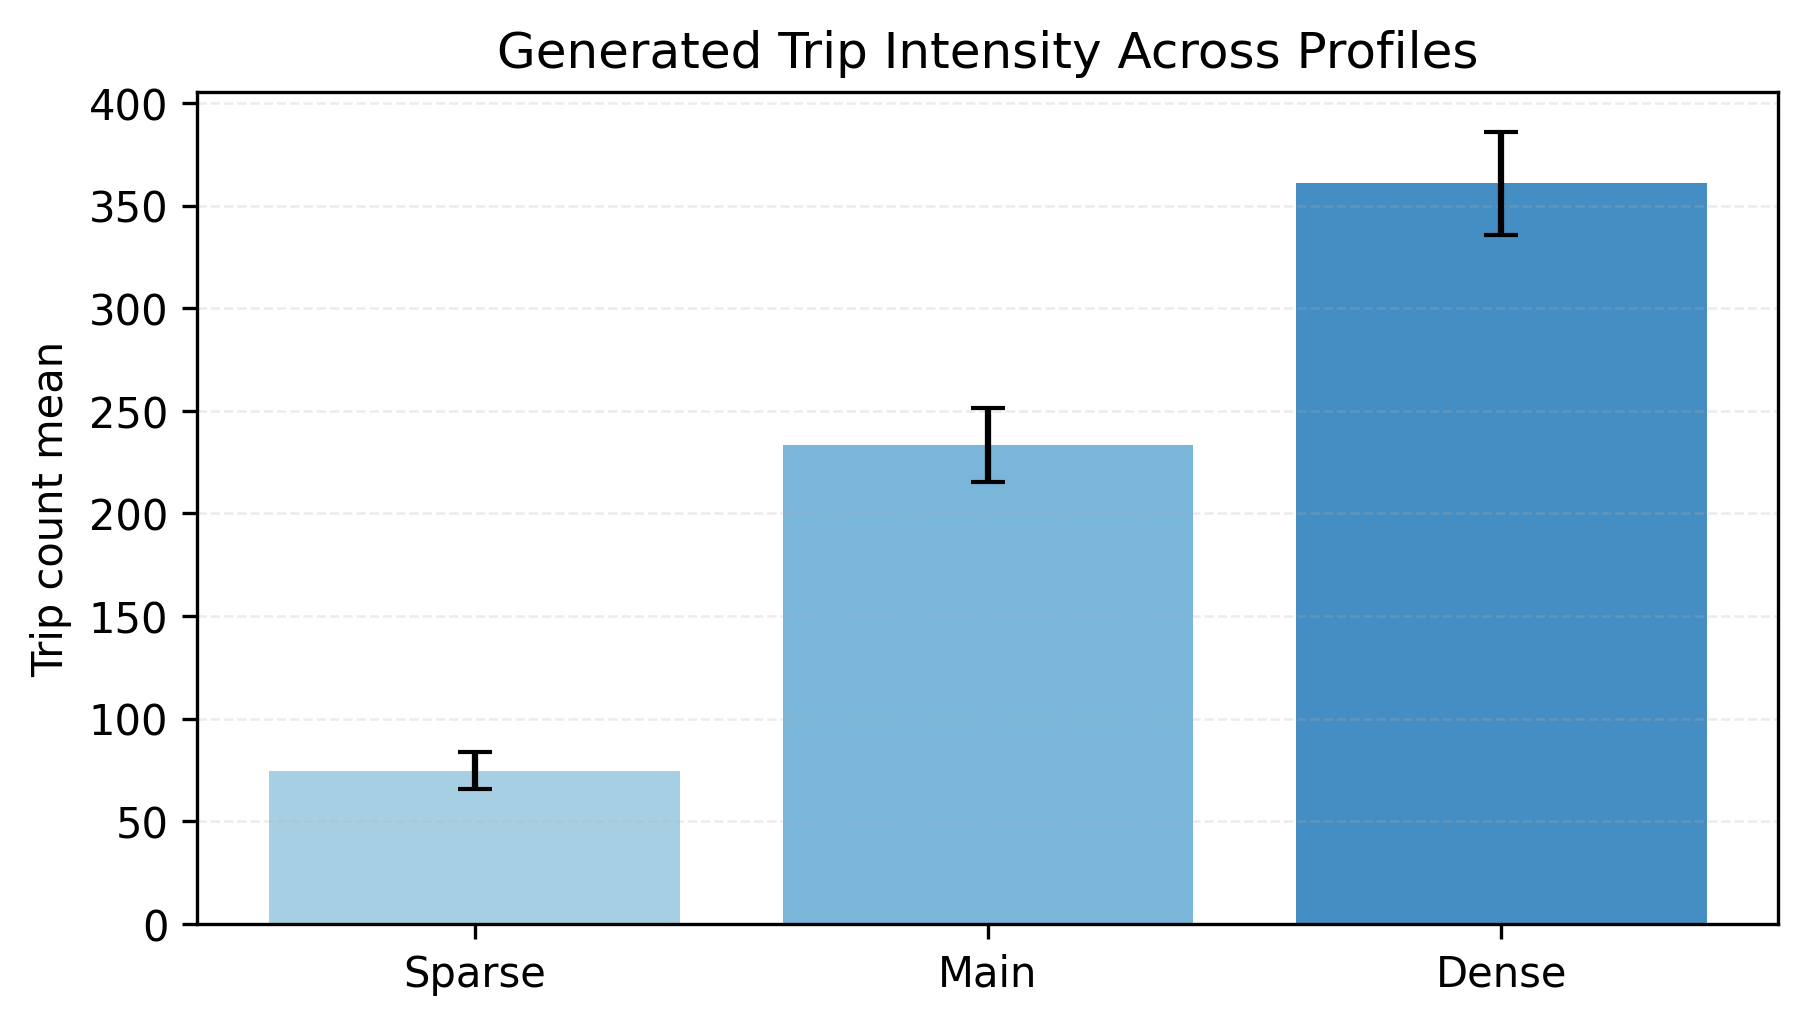
\includegraphics[width=0.86\textwidth]{figures/ch8_fig_6_2_generated_trip_intensity.png}
\caption{Generated trip intensity across sparse/main/dense profiles (error bars show one standard deviation from episode-level variance).}
\label{fig:ch8_trip_intensity_profiles}
\end{figure}

\begin{figure}[H]
\centering
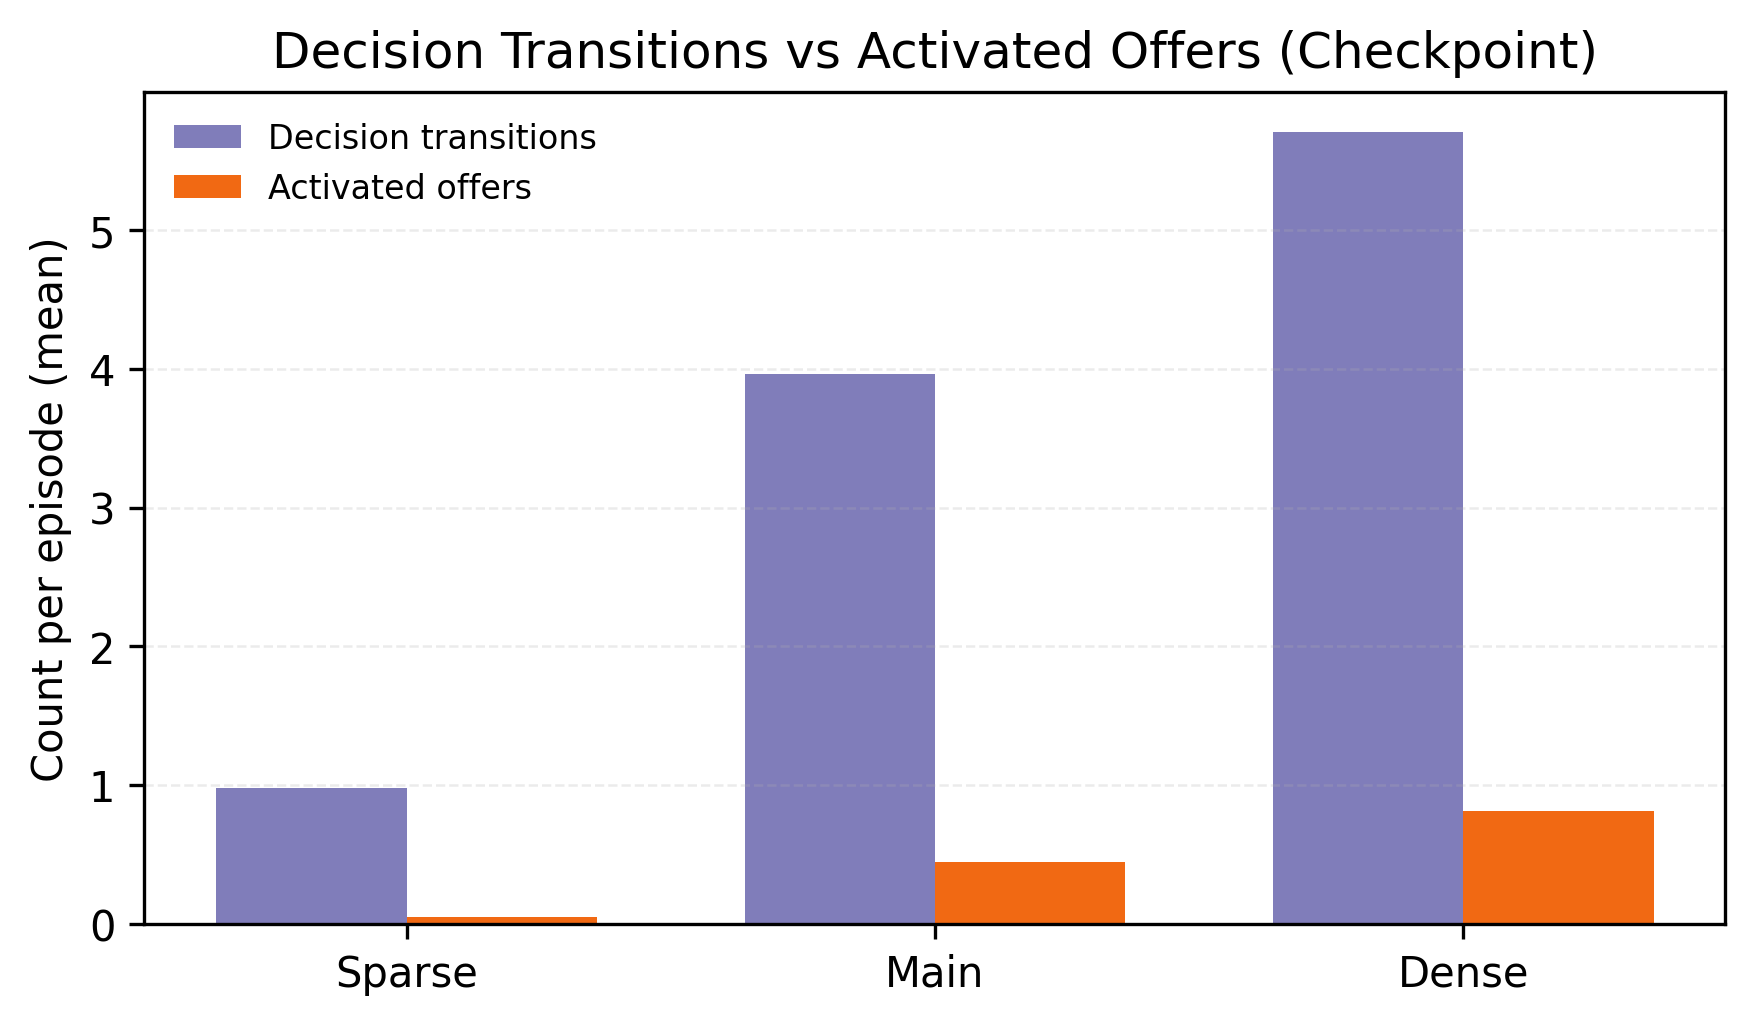
\includegraphics[width=0.86\textwidth]{figures/ch8_fig_6_3_offer_transition_density.png}
\caption{Decision transitions and activated offers across profiles under the checkpoint policy. Here, transitions denote RL state transitions (\(s,a,r,s',done\)); offers denote activated offers, not total offer opportunities.}
\label{fig:ch8_offer_transition_density}
\end{figure}

\section{Scenario 1 Results}

\subsection{Training Dynamics}

This subsection reports the learning dynamics of Scenario~1 under the final training protocol.

\begin{figure}[H]
\centering
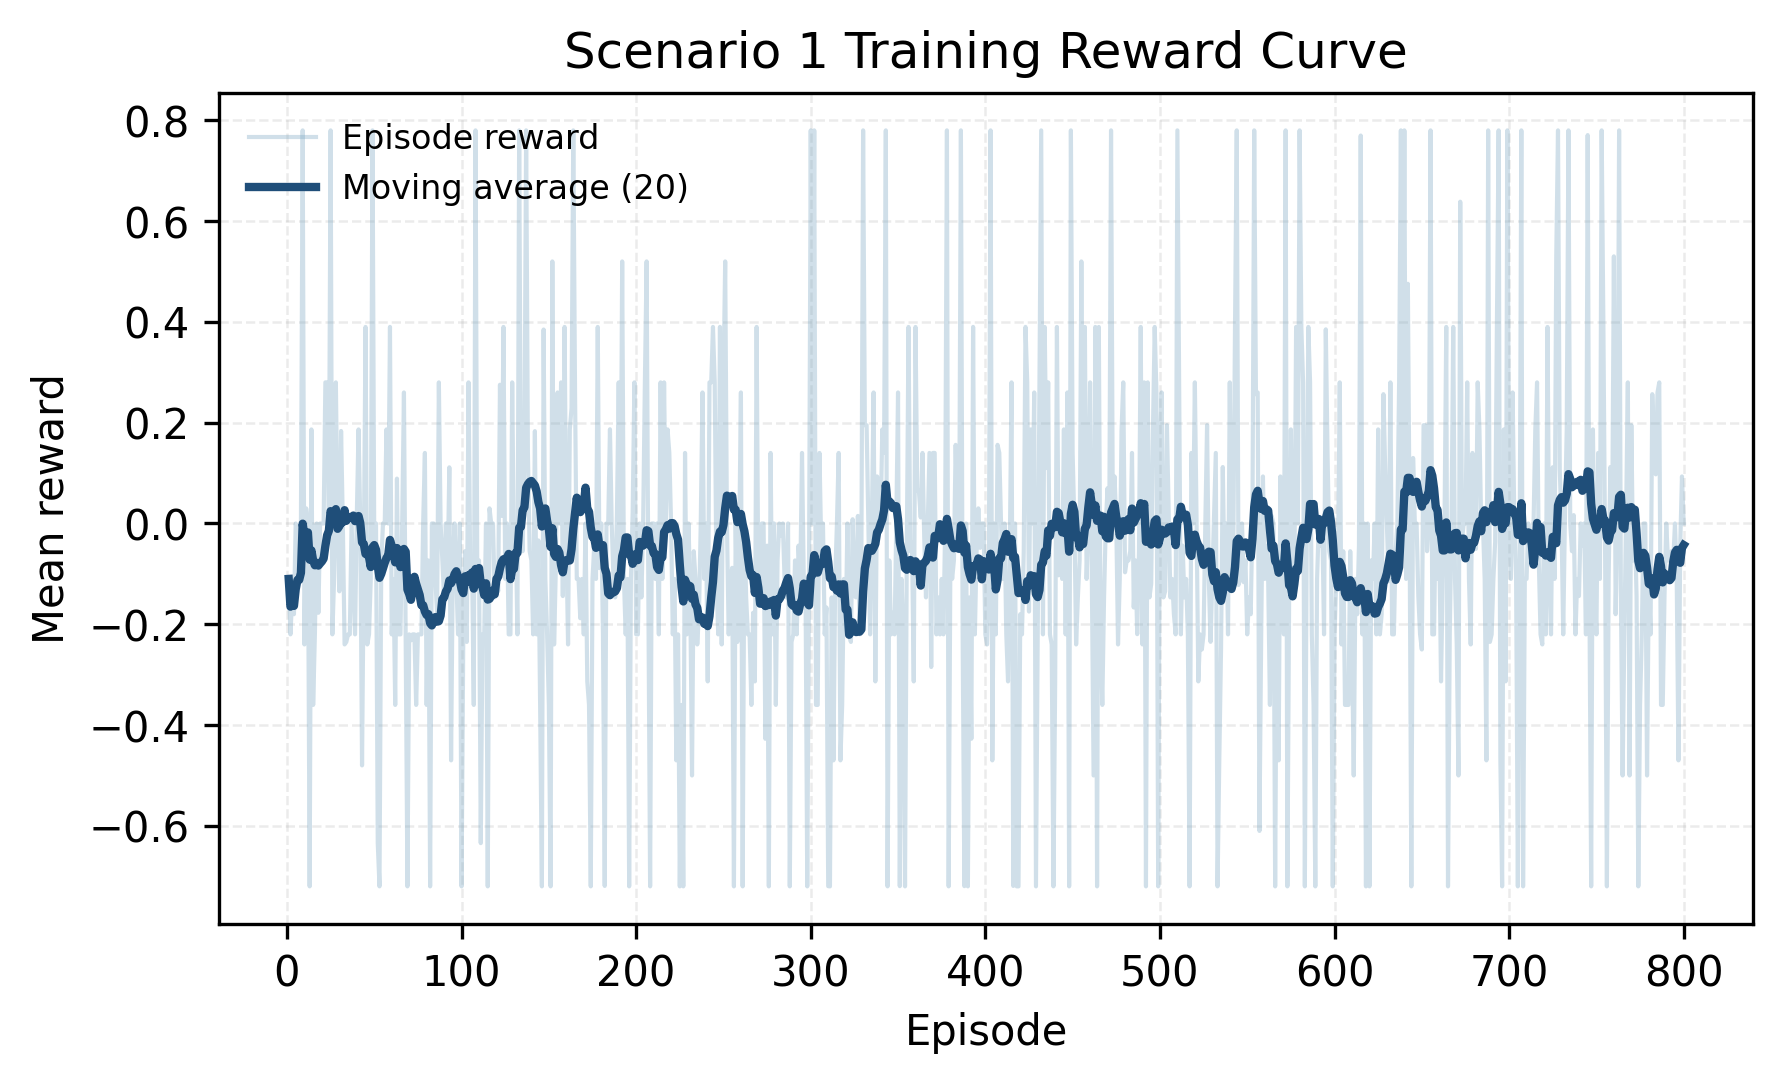
\includegraphics[width=0.9\textwidth]{figures/ch8_fig_6_4_s1_train_reward_curve.png}
\caption{Scenario~1 training reward curve (episode reward and moving average).}
\label{fig:ch8_s1_train_reward}
\end{figure}

\begin{figure}[H]
\centering
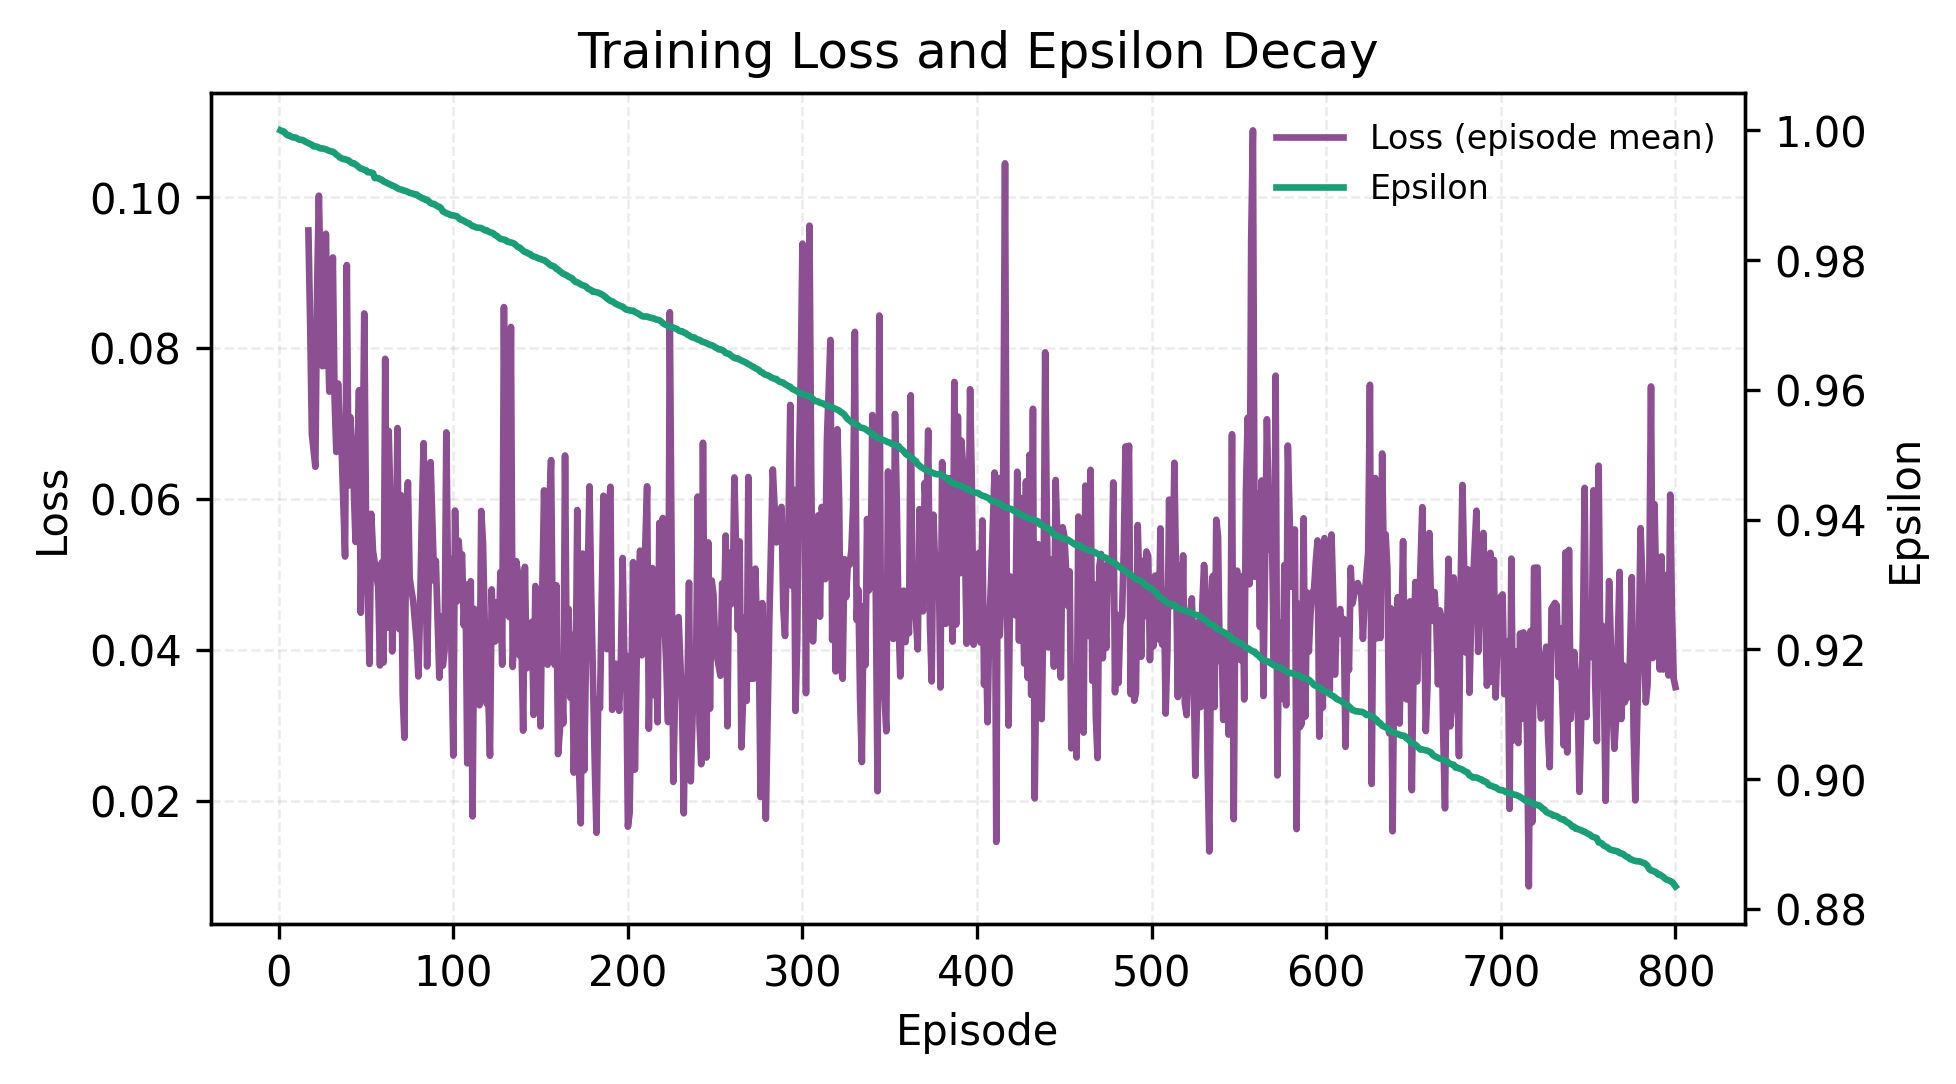
\includegraphics[width=0.9\textwidth]{figures/ch8_fig_6_5_s1_train_loss_epsilon.png}
\caption{Scenario~1 training loss and epsilon decay.}
\label{fig:ch8_s1_train_loss_epsilon}
\end{figure}

\begin{figure}[H]
\centering
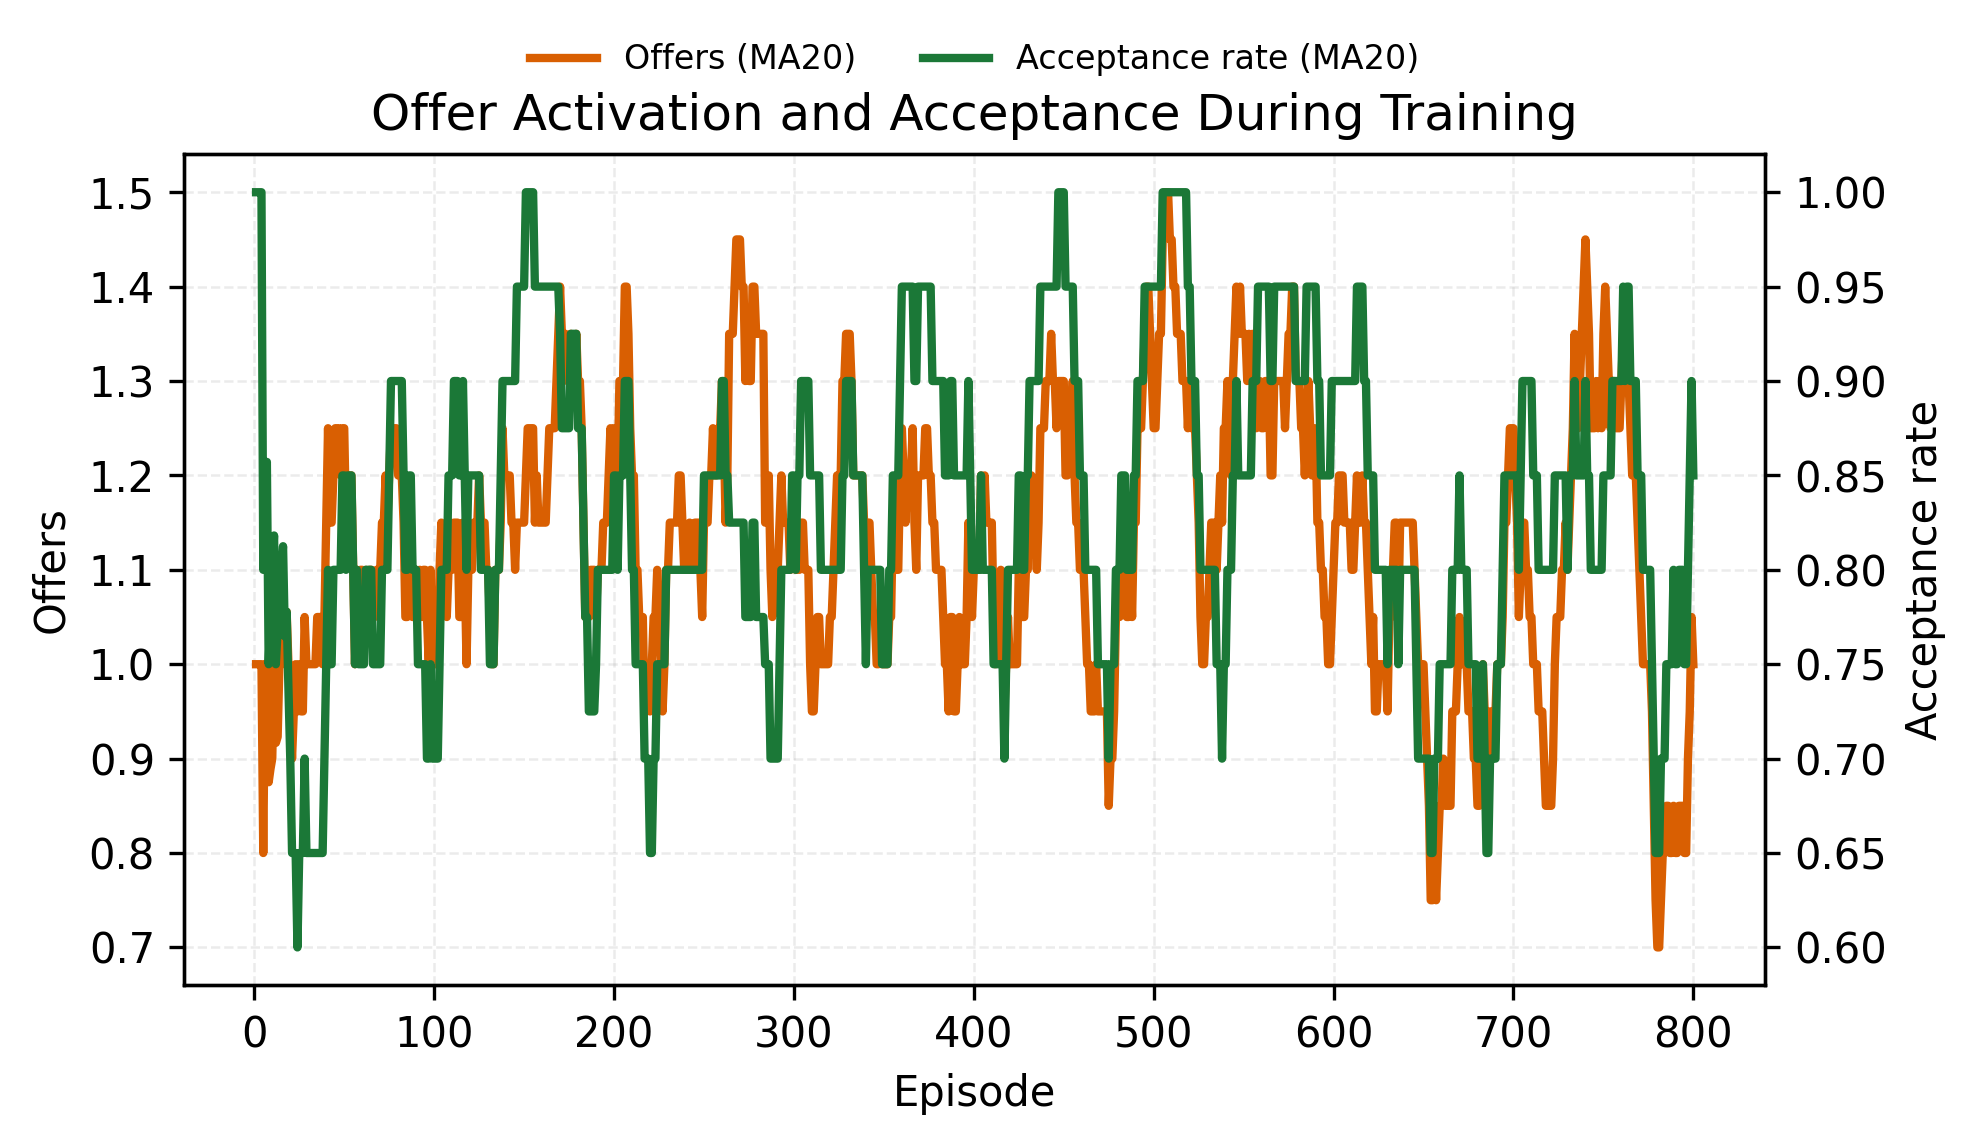
\includegraphics[width=0.9\textwidth]{figures/ch8_fig_6_6_s1_train_offers_acceptance.png}
\caption{Scenario~1 training offer activation and acceptance dynamics.}
\label{fig:ch8_s1_train_offer_accept}
\end{figure}

\begin{table}[H]
\centering
\caption{Scenario~1 training summary (last 100 episodes).}
\label{tab:ch8_s1_train_summary}
\begin{tabular}{lrrrrrr}
\toprule
Episodes & Mean reward & Std reward & Mean loss & $\epsilon_{end}$ & Mean offers & Mean accept rate \\
\midrule
100 & -0.0249 & 0.3171 & 0.0392 & 0.8835 & 1.0600 & 0.8200 \\
\bottomrule
\end{tabular}
\end{table}

Figures~\ref{fig:ch8_s1_train_reward}, \ref{fig:ch8_s1_train_loss_epsilon}, and \ref{fig:ch8_s1_train_offer_accept} show stable optimization with sustained policy activity. Table~\ref{tab:ch8_s1_train_summary} confirms that the late-stage training regime remains active and does not collapse to a trivial no-offer behavior.

\subsection{Main-Profile Policy Comparison}

Table~\ref{tab:ch8_main_policy} reports the primary comparison under the \textit{main} profile. Compared with fixed policies, the checkpoint policy achieves the highest mean reward while maintaining comparable service rate.

\begin{table}[H]
\centering
\caption{Main-profile policy comparison (Scenario~1).}
\label{tab:ch8_main_policy}
\small
\setlength{\tabcolsep}{4pt}
\resizebox{\textwidth}{!}{%
\begin{tabular}{lrrrrrrrr}
\toprule
Policy & Service rate (mean $\pm$ std) & Offers & Accepted & Acceptance rate & Mean reward (mean $\pm$ std) & Mean realized loss & Mean $\Delta EDL$ (mean $\pm$ std) & Mean transitions \\
\midrule
No-offer     & 0.9639 $\pm$ 0.0243 & 0.0225 & 0.0000 & 0.0000 $\pm$ 0.0000 & -0.0253 $\pm$ 0.0861 & 0.1667 & 0.0000 $\pm$ 0.0000 & 4.8725 \\
Always-offer & 0.9644 $\pm$ 0.0245 & 1.4625 & 1.4425 & 0.9157 $\pm$ 0.2750 & -0.0752 $\pm$ 0.4196 & 0.8425 & -0.1248 $\pm$ 0.1374 & 1.4425 \\
Checkpoint   & 0.9644 $\pm$ 0.0244 & 0.4475 & 0.4250 & 0.3779 $\pm$ 0.4851 & 0.1154 $\pm$ 0.2731 & 0.2854 & 0.0091 $\pm$ 0.0190 & 3.9650 \\
\bottomrule
\end{tabular}
}
\end{table}

Under the main profile, the checkpoint policy is more selective than \textit{always-offer} (fewer offers and fewer accepted relocations) and avoids its negative EDL trend. Relative to \textit{no-offer}, checkpoint activates additional offers and converts that activity into positive mean reward. Figure~\ref{fig:ch8_main_kpi_comparison} shows this policy separation visually.

\begin{figure}[H]
\centering
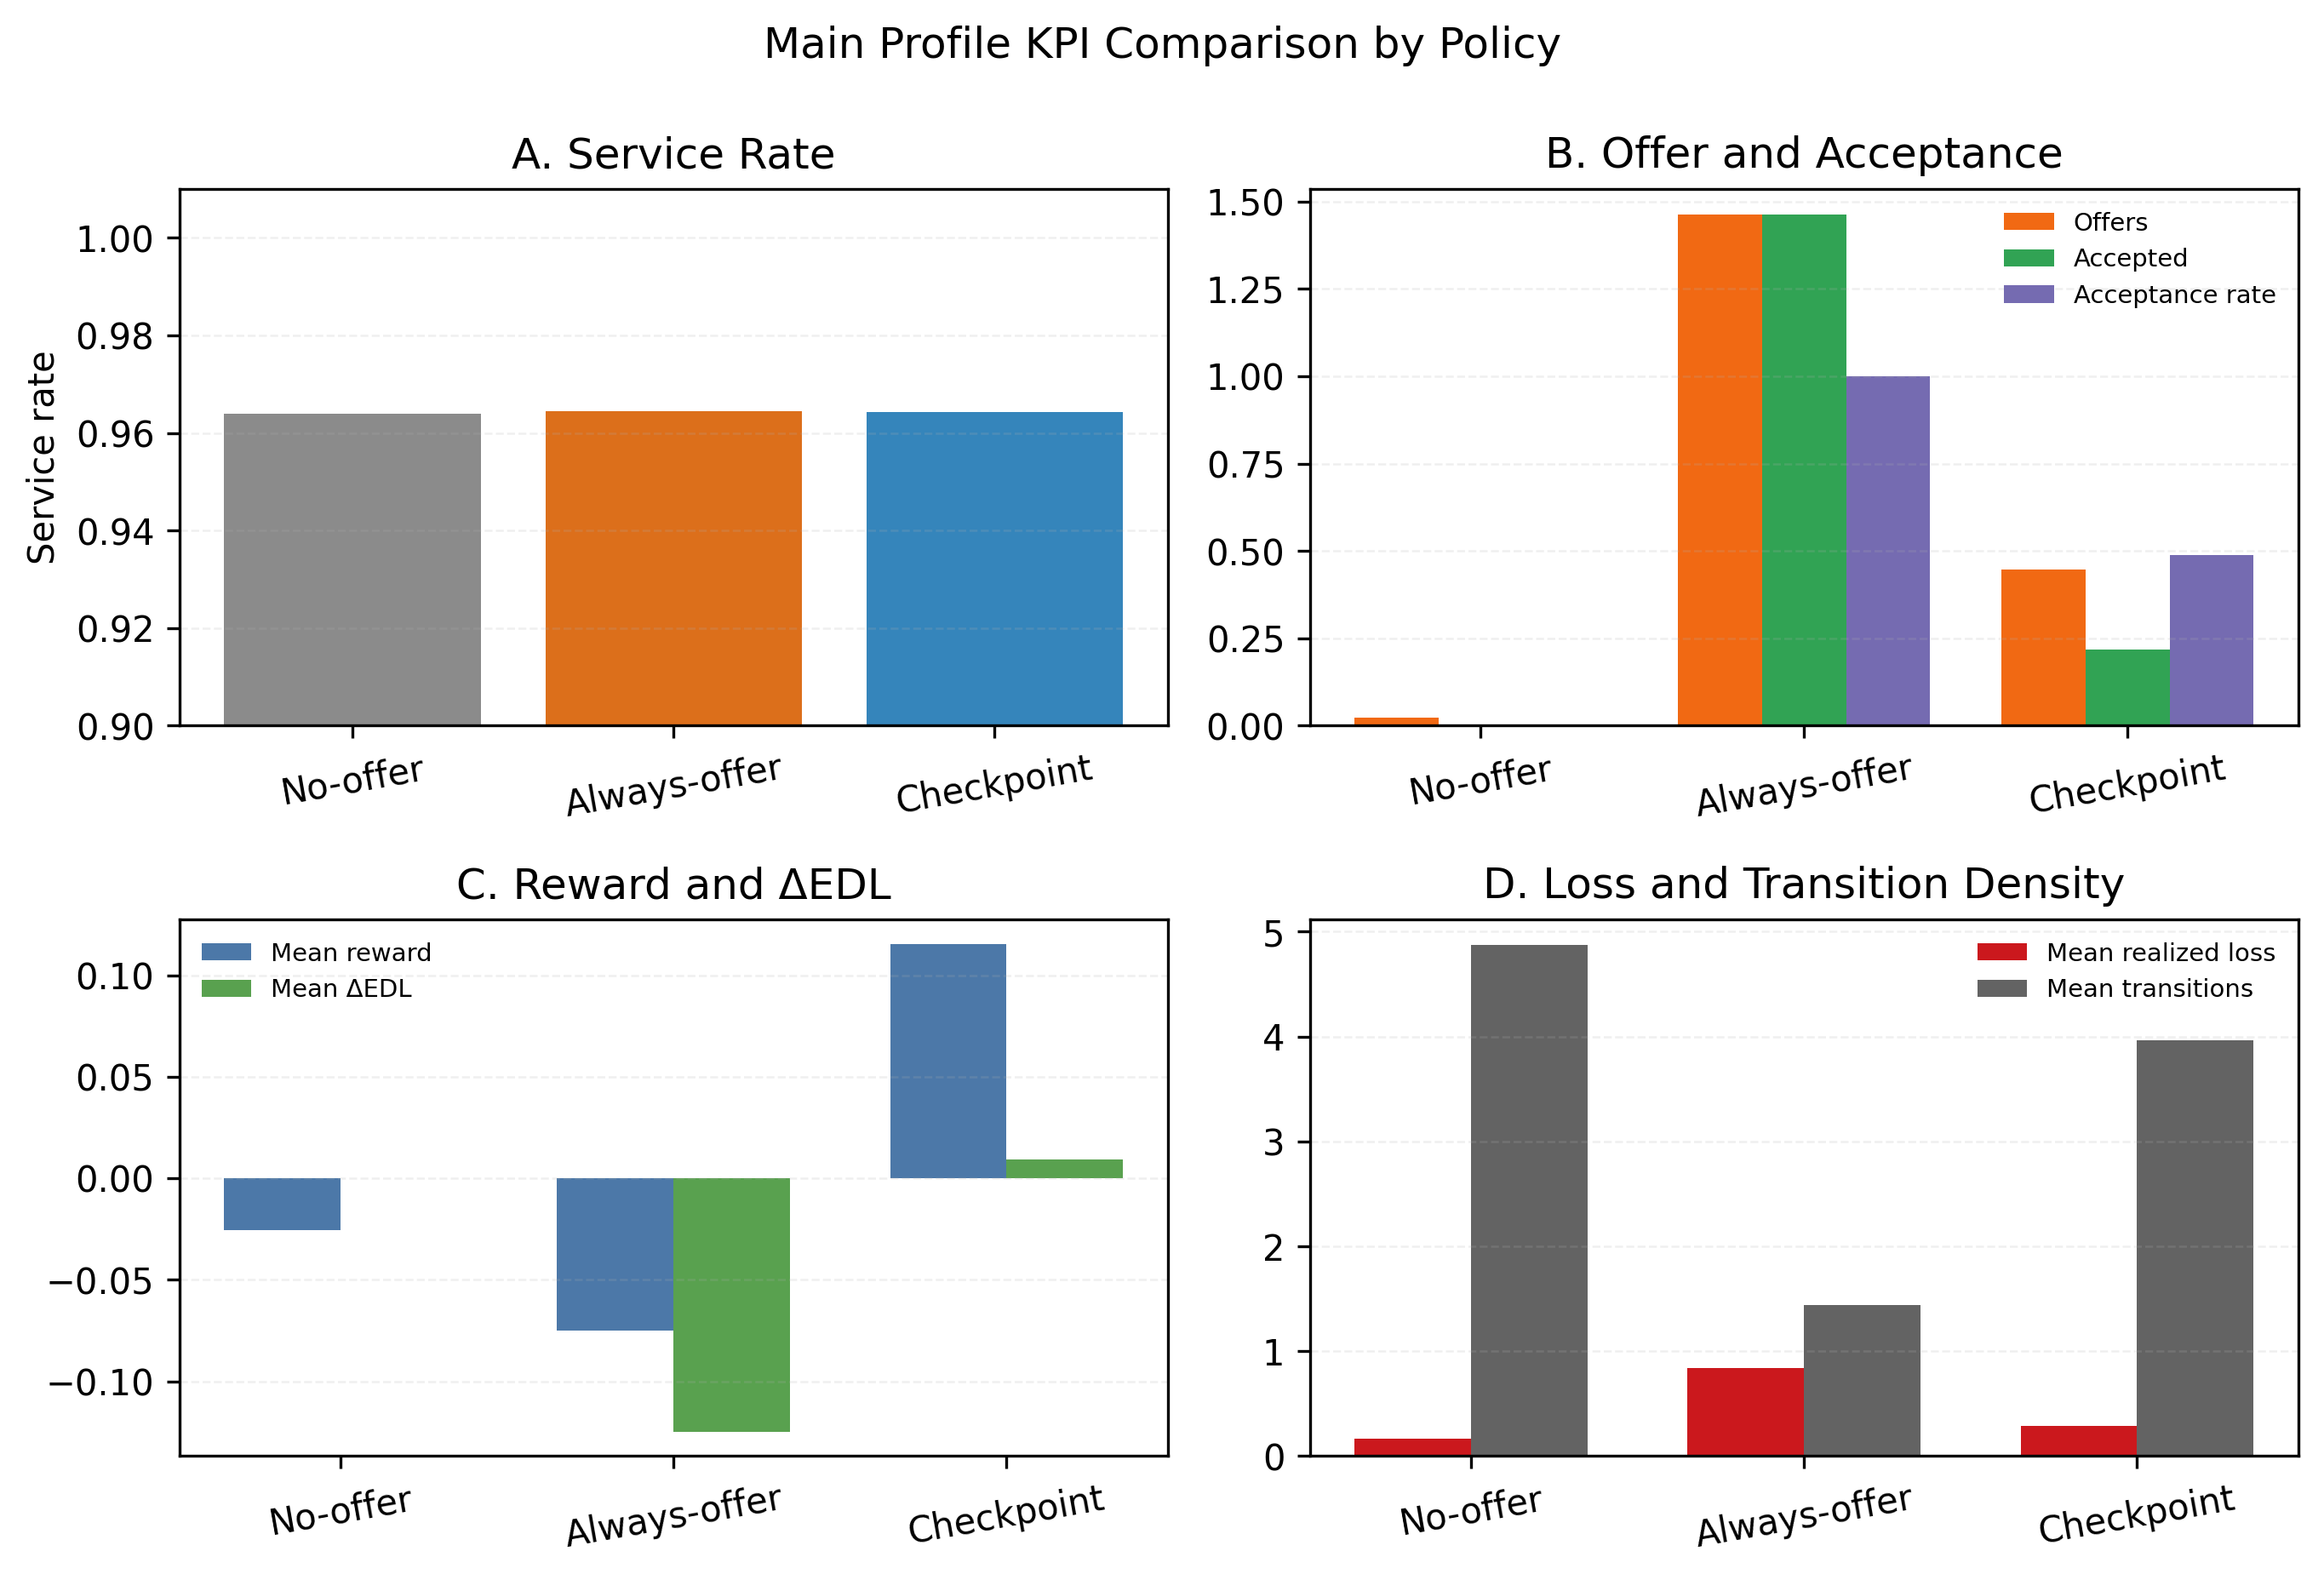
\includegraphics[width=0.9\textwidth]{figures/ch8_fig_6_7_main_profile_kpi_comparison.png}
\caption{Main-profile KPI comparison across no-offer, always-offer, and checkpoint policies (2x2 panel: service rate; offer/acceptance behavior; reward and $\Delta EDL$; realized-loss and transition density).}
\label{fig:ch8_main_kpi_comparison}
\end{figure}

\subsection{Robustness Across Sparse/Main/Dense Profiles}

Table~\ref{tab:ch8_robustness_three_profiles} summarizes the same policy trio across all three profiles.

\begin{table}[H]
\centering
\caption{Policy comparison across sparse/main/dense profiles (Scenario~1).}
\label{tab:ch8_robustness_three_profiles}
\small
\setlength{\tabcolsep}{4pt}
\resizebox{\textwidth}{!}{%
\begin{tabular}{llrrrrr}
\toprule
Profile & Policy & Service rate (mean $\pm$ std) & Offers & Mean reward (mean $\pm$ std) & Mean $\Delta EDL$ (mean $\pm$ std) & Mean realized loss \\
\midrule
Sparse & No-offer     & 0.9984 $\pm$ 0.0057 & 0.0000 & 0.0000 $\pm$ 0.0000  & 0.0000 $\pm$ 0.0000  & 0.0000 \\
Sparse & Always-offer & 0.9991 $\pm$ 0.0045 & 0.6600 & -0.0832 $\pm$ 0.1995 & -0.0929 $\pm$ 0.1160 & 0.0025 \\
Sparse & Checkpoint   & 0.9985 $\pm$ 0.0056 & 0.0525 & 0.0305 $\pm$ 0.1443  & 0.0016 $\pm$ 0.0082  & 0.0000 \\
\midrule
Main & No-offer       & 0.9639 $\pm$ 0.0243 & 0.0225 & -0.0253 $\pm$ 0.0861 & 0.0000 $\pm$ 0.0000  & 0.1667 \\
Main & Always-offer   & 0.9644 $\pm$ 0.0245 & 1.4625 & -0.0752 $\pm$ 0.4196 & -0.1248 $\pm$ 0.1374 & 0.8425 \\
Main & Checkpoint     & 0.9644 $\pm$ 0.0244 & 0.4475 & 0.1154 $\pm$ 0.2731  & 0.0091 $\pm$ 0.0190  & 0.2854 \\
\midrule
Dense & No-offer      & 0.9104 $\pm$ 0.0339 & 0.0450 & -0.0529 $\pm$ 0.0996 & 0.0000 $\pm$ 0.0000  & 0.6904 \\
Dense & Always-offer  & 0.9088 $\pm$ 0.0354 & 1.6925 & -0.1098 $\pm$ 0.4395 & -0.0938 $\pm$ 0.1288 & 4.2175 \\
Dense & Checkpoint    & 0.9100 $\pm$ 0.0346 & 0.8125 & 0.0971 $\pm$ 0.2649  & 0.0133 $\pm$ 0.0336  & 1.8940 \\
\bottomrule
\end{tabular}
}
\end{table}

Three robustness observations are consistent across profiles:
\begin{itemize}
\item checkpoint mean reward remains positive in all three profiles;
\item checkpoint mean $\Delta EDL$ remains positive, while \textit{always-offer} is negative;
\item checkpoint preserves service rate close to fixed-policy baselines without over-activating offers.
\end{itemize}

As shown in Figures~\ref{fig:ch8_reward_edl_robustness} and \ref{fig:ch8_offers_robustness}, seed-level dispersion increases from sparse to dense, which is consistent with stronger demand uncertainty under denser profile settings.

\begin{figure}[H]
\centering
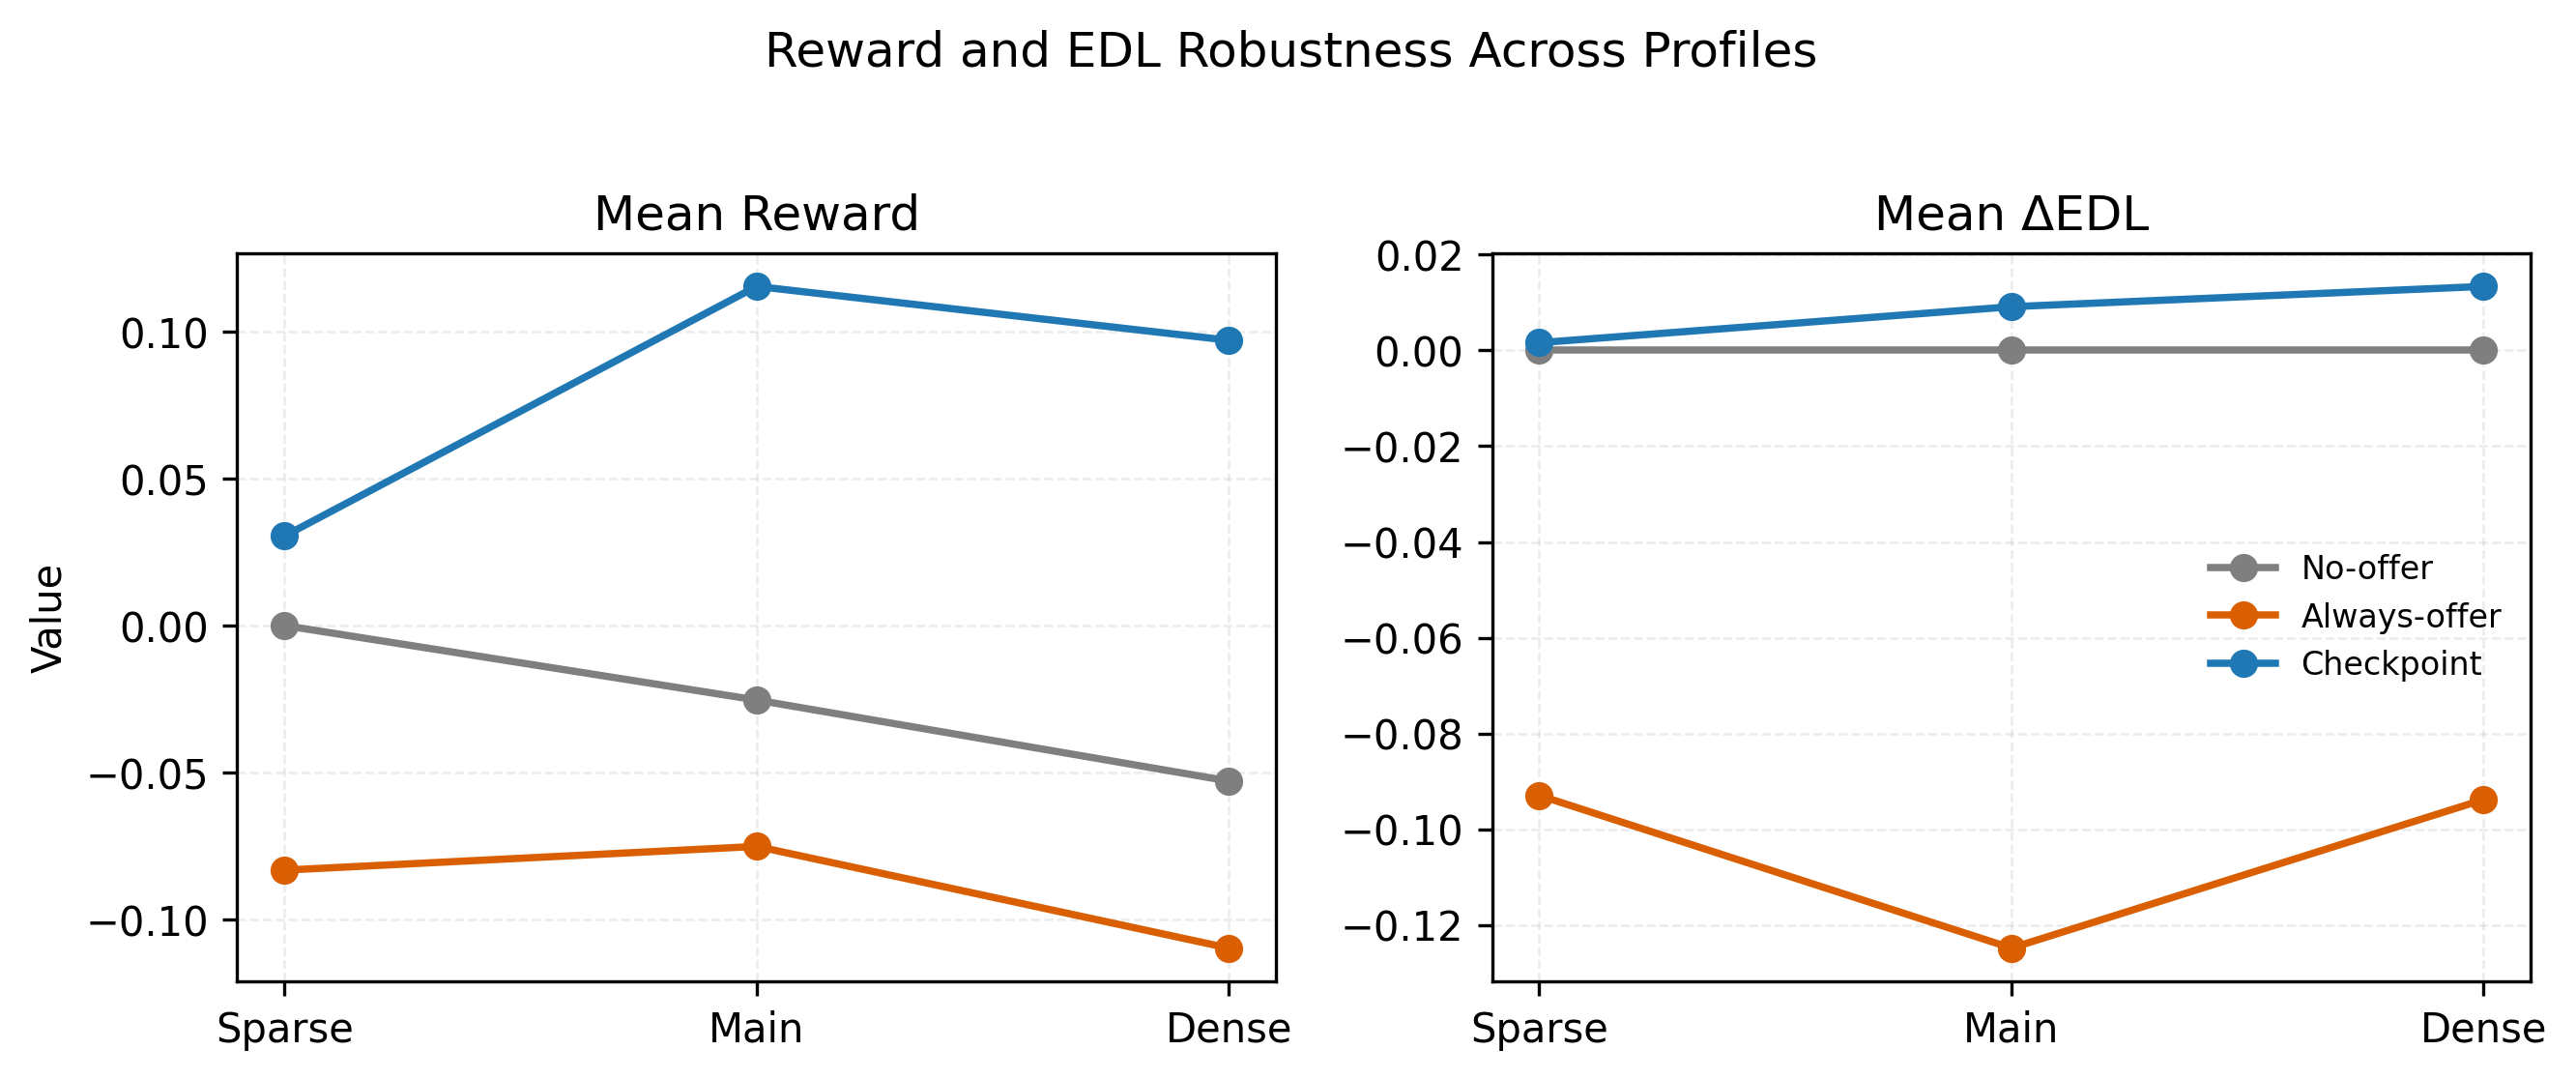
\includegraphics[width=0.9\textwidth]{figures/ch8_fig_6_8_reward_edl_robustness.png}
\caption{Reward and $\Delta EDL$ robustness across sparse/main/dense profiles.}
\label{fig:ch8_reward_edl_robustness}
\end{figure}

\begin{figure}[H]
\centering
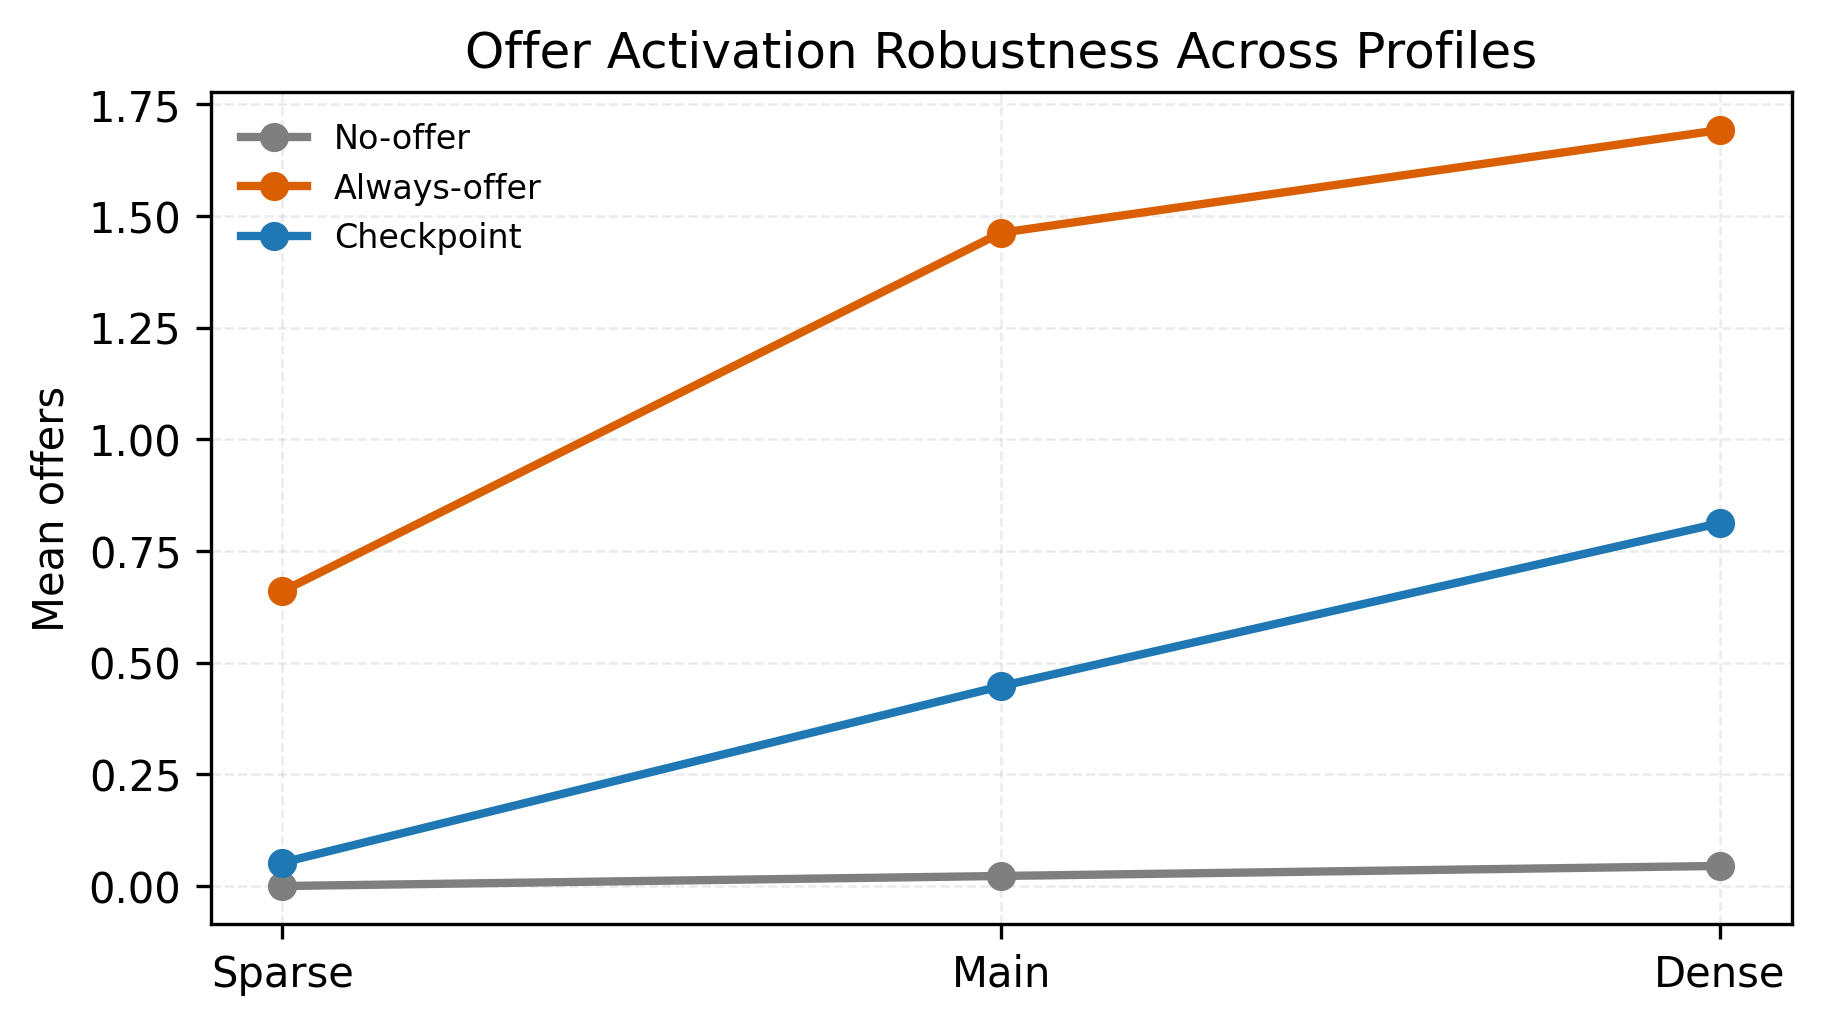
\includegraphics[width=0.9\textwidth]{figures/ch8_fig_6_9_offers_robustness.png}
\caption{Offer-activation robustness across sparse/main/dense profiles.}
\label{fig:ch8_offers_robustness}
\end{figure}

\subsection{Reward Decomposition}

To interpret policy behavior, Table~\ref{tab:ch8_reward_decomp_main} reports reward-component means under the \textit{main} profile.

\begin{table}[H]
\centering
\caption{Reward decomposition by policy in the main profile (Scenario~1).}
\label{tab:ch8_reward_decomp_main}
\begin{tabular}{lrrrr}
\toprule
Policy & Mean reward realized term & Mean reward EDL term & Mean reward accept term & Mean reward \\
\midrule
No-offer     & -0.0253 & 0.0000  & 0.0000 & -0.0253 \\
Always-offer & -0.1094 & -0.2234 & 0.3680 & -0.0752 \\
Checkpoint   & -0.0405 & 0.0949  & 0.0872 & 0.1154 \\
\bottomrule
\end{tabular}
\end{table}

The decomposition indicates that checkpoint performance is not driven by acceptance reward alone. The positive EDL component is a central contributor, and the realized-loss penalty remains materially lower than in \textit{always-offer}. Figure~\ref{fig:ch8_reward_component_breakdown} provides the signed contribution view of each reward component.

\begin{figure}[H]
\centering
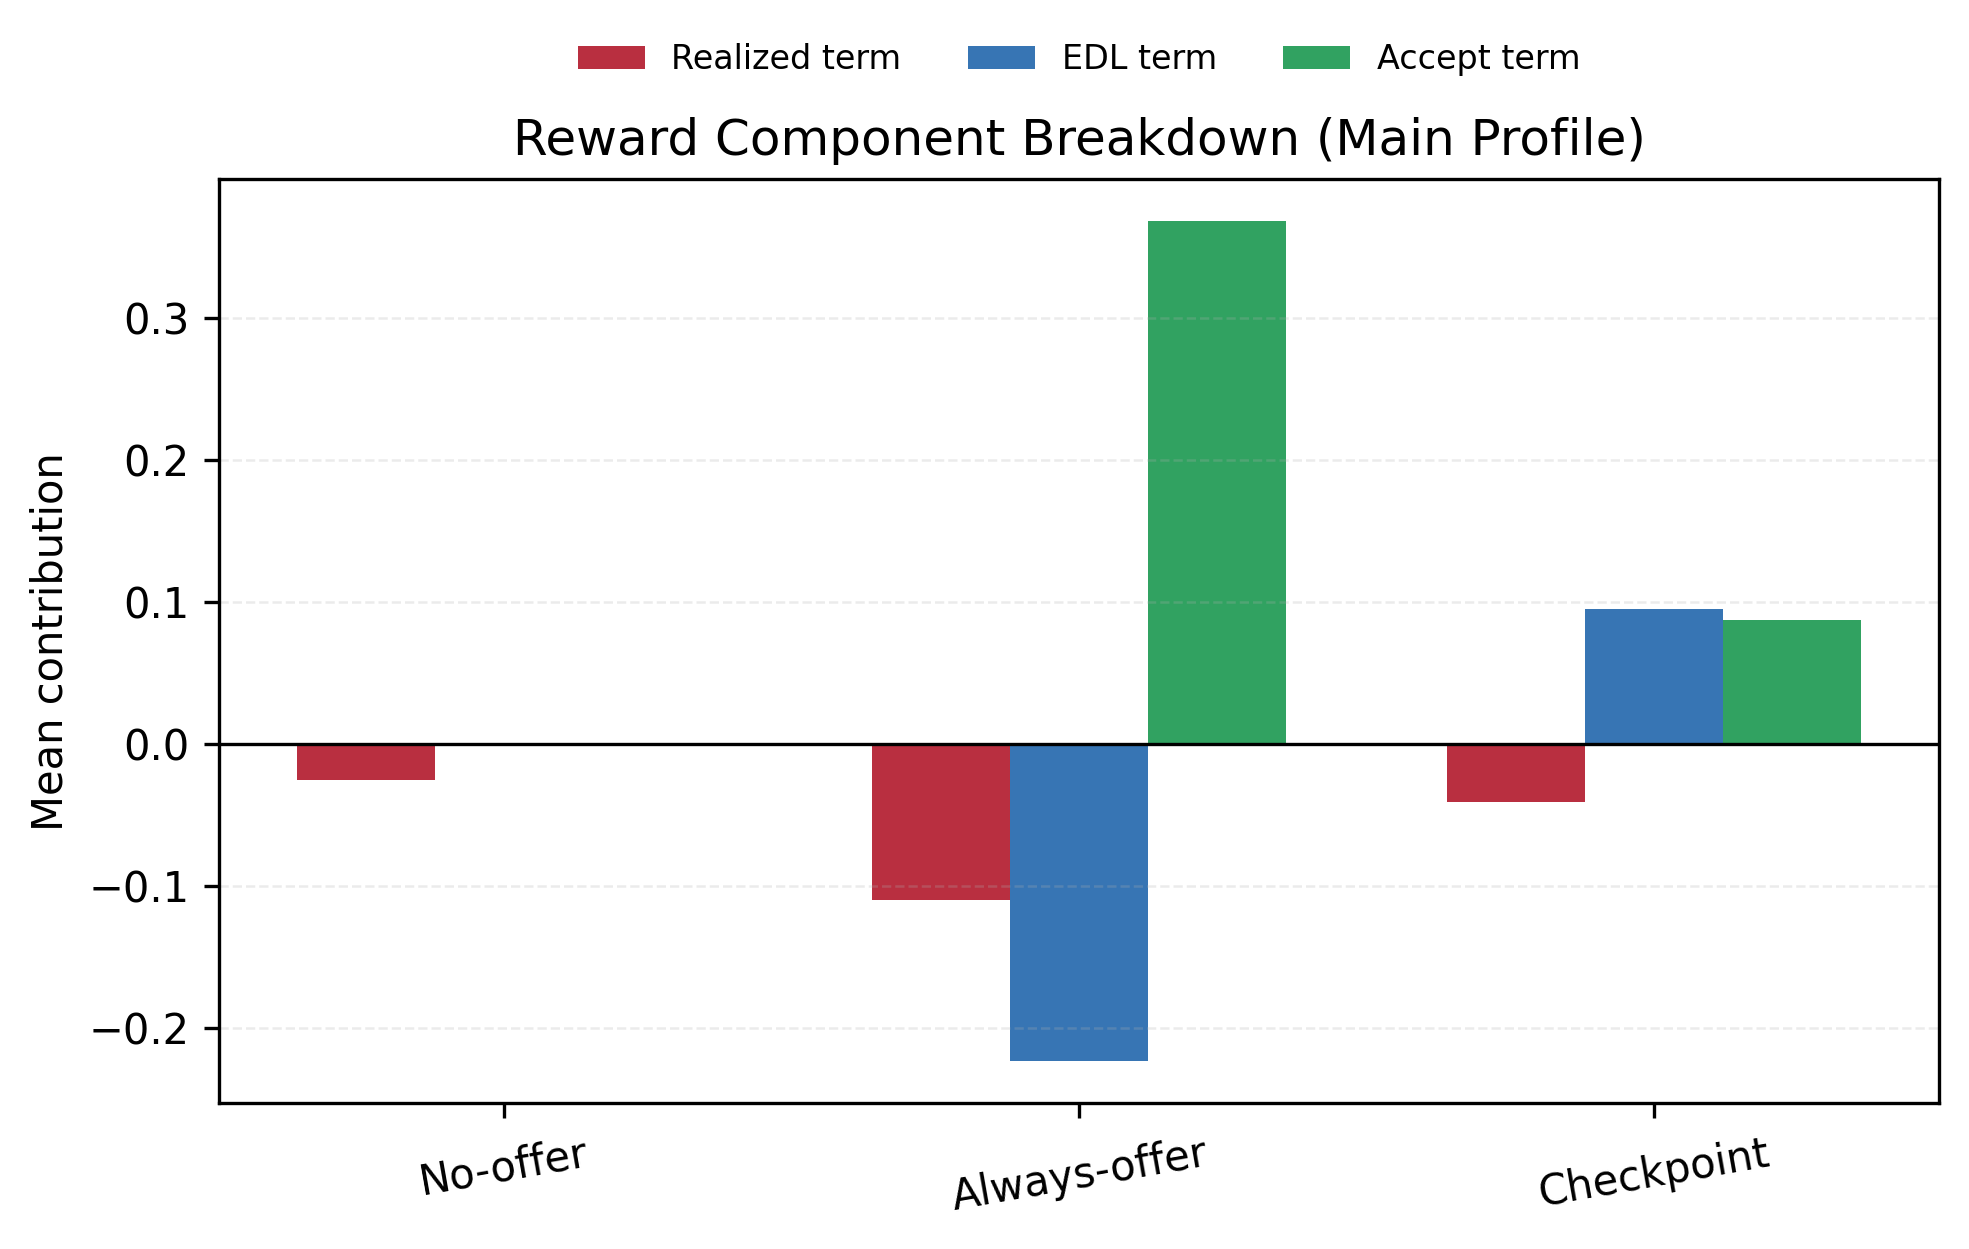
\includegraphics[width=0.9\textwidth]{figures/ch8_fig_6_10_reward_component_breakdown.png}
\caption{Main-profile reward component breakdown by policy.}
\label{fig:ch8_reward_component_breakdown}
\end{figure}

\subsection{Sensitivity Analysis (Placeholder)}

\textit{\detokenize{<TAB_6_5_S1_SENSITIVITY_MATRIX>}}

\textit{\detokenize{<FIG_6_11_S1_SENSITIVITY_RANKING>}}

\textit{This subsection reports targeted sensitivity results for reward parameters and demand-profile settings.}

\section{Scenario 2 Results}

\subsection{Training Dynamics}
\textit{\detokenize{<TAB_6_6_S2_TRAINING_SUMMARY>}}

\textit{\detokenize{<FIG_6_12_S2_TRAINING_CURVES>}}

\subsection{Main-Profile Policy Comparison}
\textit{\detokenize{<TAB_6_7_S2_MAIN_POLICY_COMPARISON>}}

\textit{\detokenize{<FIG_6_13_S2_OPTION_ACTION_DISTRIBUTION>}}

\subsection{Robustness Across Profiles}
\textit{\detokenize{<TAB_6_8_S2_ROBUSTNESS_PROFILES>}}

\textit{\detokenize{<FIG_6_14_S2_ROBUSTNESS_REWARD_EDL>}}

\subsection{Reward Decomposition and Operational Interpretation}
\textit{\detokenize{<TAB_6_9_S2_REWARD_DECOMPOSITION>}}

\textit{\detokenize{<FIG_6_15_S2_REWARD_COMPONENT_BREAKDOWN>}}

\subsection{Sensitivity Analysis}
\textit{\detokenize{<TAB_6_10_S2_SENSITIVITY_MATRIX>}}

\textit{\detokenize{<FIG_6_16_S2_SENSITIVITY_RANKING>}}

\section{Cross-Scenario Comparison}

Cross-scenario comparison follows an aligned metric schema so that Scenario~1 and Scenario~2 can be interpreted under the same operational and reward dimensions.

\begin{table}[H]
\centering
\caption{Cross-scenario comparison structure (aligned schema).}
\label{tab:ch8_cross_scenario}
\begin{tabular}{lcc}
\toprule
Dimension & Scenario~1 & Scenario~2 \\
\midrule
Action space & Binary offer activation & \texttt{\detokenize{<S2_ACTION_SPACE_DESC>}} \\
Training results & Reported & \texttt{\detokenize{<S2_TRAINING_STATUS_TOKEN>}} \\
Main-profile evaluation & Reported & \texttt{\detokenize{<S2_MAIN_EVAL_STATUS_TOKEN>}} \\
Robustness evaluation & Reported & \texttt{\detokenize{<S2_ROBUSTNESS_STATUS_TOKEN>}} \\
Sensitivity evaluation & \texttt{\detokenize{<S1_SENS_STATUS_TOKEN>}} & \texttt{\detokenize{<S2_SENS_STATUS_TOKEN>}} \\
\bottomrule
\end{tabular}
\end{table}

\textbf{Figure placeholder (position reserved):}
\begin{itemize}
\item \texttt{\detokenize{<FIG_6_17_CROSS_SCENARIO_COMPARISON>}}
\end{itemize}

\section{Findings Mapped to Research Questions}

\subsection*{RQ1: Execution mismatch identification}
The results confirm that downstream execution policies produce distinct outcomes even with fixed OR outputs. This supports the relevance of the planning-execution mismatch studied in this thesis.

\subsection*{RQ2: Decision-mechanism design}
The Scenario~1 binary refinement mechanism is operationally feasible and produces stable comparative outputs under unified evaluation settings.

\subsection*{RQ3: Comparative performance}
Across sparse/main/dense profiles, checkpoint consistently dominates \textit{always-offer} in reward and EDL direction while maintaining comparable service rate, indicating that selective activation is preferable to unconditional activation in the current setup.

\section{Chapter Summary}

This chapter reports results using one unified protocol across two scenarios, three policies, and three demand profiles. Scenario~1 numerical evidence is provided through consistent table-based reporting, and Scenario~2 uses aligned placeholders to preserve full structural comparability for direct result insertion in the next revision.

\textbf{Figure placeholder (position reserved):}
\begin{itemize}
\item \texttt{\detokenize{<FIG_6_18_CHAPTER_KEY_FINDINGS_SNAPSHOT>}}
\end{itemize}

\chapter{Discussion}
\label{chapter:discussion}

This chapter interprets the empirical results, explains the mechanisms behind the main patterns observed in the experiments, and reflects on the broader implications and limitations of the proposed refinement layer.

\section{Interpretation of Main Findings}

This section explains when and why the refinement layer improves outcomes, and where those gains remain limited under the current design.

\section{Relation to Prior Literature}

This section positions the empirical findings relative to the literature reviewed in Chapter~\ref{chapter:literature-review}, with particular attention to the planning--execution interface, RL-based operational control, and user-incentive design.

\section{Operational and Managerial Implications}

This section discusses what the results imply for incentive policy design, execution governance, budget allocation, and the practical deployment of trip-level refinement policies in shared micromobility systems.

\section{Limitations}

This section reflects on the main limitations of the current study, including model assumptions, data constraints, scenario simplifications, and questions of external validity.

\section{Future Work}

This section outlines concrete next steps, including broader scenario design, richer action spaces, tighter integration with upstream planning models, and possible extensions toward online or field deployment.

\chapter{Conclusion}
\label{chapter:conclusion}

This chapter concludes the thesis by summarizing answers to the research questions and outlining practical and scientific takeaways.

\section{Answers to the Research Questions}
Provide concise answers to the main research question and RQ1-RQ3 based on the evidence presented.

\section{Scientific Contribution}
Summarize methodological and empirical contributions of the thesis.

\section{Practical Implications}
State how the findings can inform real-world shared micromobility operations.

\section{Final Remarks}
Close with the boundary of current findings and a short outlook on extension potential.


%% Prevent urls running into margins in bibliography
\setcounter{biburlnumpenalty}{7000}
\setcounter{biburllcpenalty}{7000}
\setcounter{biburlucpenalty}{7000}

%% Add bibliography
\printbibliography[heading=bibintoc,title=References]

%% ----------------------------------------------------------------------
%%    Appendix (Letters for chapters)
%% ----------------------------------------------------------------------

\appendix

\input{appendix/appendix-a}
\input{appendix/appendix-b}
%\input{appendix/appendix-c} % Create file to add

\end{document}

